\documentclass[12pt,a4paper]{article}

\usepackage[a4paper,margin=1in]{geometry}
\usepackage{graphicx}
\usepackage{booktabs}
\usepackage{amsmath,amssymb}
\usepackage{float}
\usepackage{hyperref}
\usepackage{xurl}
\usepackage{xcolor}
\usepackage{listings}
\usepackage{enumitem}
\usepackage{fancyhdr}
\usepackage{longtable}
\usepackage{array}

\hypersetup{colorlinks=true,linkcolor=blue,urlcolor=blue,citecolor=blue}

\pagestyle{fancy}
\fancyhf{}
\setlength{\headheight}{15pt}
\lhead{ICS1512}
\rhead{Machine Learning Algorithms Laboratory}
\cfoot{\thepage}

\graphicspath{{./}{figures/}}

\setlength{\parskip}{0.35em}
\setlength{\parindent}{0pt}

\setlength{\floatsep}{6pt plus 2pt minus 2pt}
\setlength{\textfloatsep}{8pt plus 2pt minus 2pt}
\setlength{\intextsep}{6pt plus 2pt minus 2pt}

\lstset{
  language=Python,
  basicstyle=\ttfamily\footnotesize,
  numbers=left,
  frame=single,
  breaklines=true,
  showstringspaces=false,
  keywordstyle=\color{blue},
  commentstyle=\color{gray},
  stringstyle=\color{teal}
}

\begin{document}

\noindent
\resizebox{\linewidth}{!}{%
\begin{tabular}{|p{4.2cm}|p{11.8cm}|}
\hline
Experiment No. & 8 \\ \hline
Experiment Title & Clustering Human Activity Recognition Data using K-Means, DBSCAN, and Hierarchical Clustering \\ \hline
GitHub Repository & \url{https://github.com/Srinivasan1716/Machine_Learning_Course} \\ \hline
Student Name & Srinivasan M \\ \hline
Register Number & 3122247001063 \\ \hline
Faculty & Dr. Poreddy Ajay Kumar Reddy \\ \hline
Submission Date & September 21, 2026 \\ \hline
\end{tabular}%
}

\vspace{0.4cm}

\section{Objective}
The primary objectives of this laboratory experiment are:
\begin{itemize}[noitemsep]
    \item To implement, optimize, and systematically analyze three foundational unsupervised clustering algorithms on the \textbf{Human Activity Recognition (HAR) Using Smartphones Dataset}:
    \begin{enumerate}[label=(\alph*),noitemsep]
        \item \textbf{Model A: K-Means Clustering} (Centroid-based spatial partitioning with Lloyd's optimization).
        \item \textbf{Model B: DBSCAN} (Density-Based Spatial Clustering of Applications with Noise).
        \item \textbf{Model C: Hierarchical Agglomerative Clustering (HAC)} (Bottom-up agglomerative linkage merging).
    \end{enumerate}
    \item To investigate the \textbf{Elbow Method} across cluster candidates $k \in \{2, 3, 4, 5, 6, 7, 8\}$ by recording Within-Cluster Sum of Squares (WCSS/Inertia) and Mean Silhouette Scores, and to theoretically justify the selection of optimal $k$.
    \item To tune DBSCAN parameters ($\epsilon$ neighborhood radius and $\text{minPts}$) using the $k$-nearest neighbor distance knee heuristic under principal component subspace projection.
    \item To generate hierarchical tree dendrograms using Ward's minimum variance linkage, and comparatively analyze Cophenetic correlation coefficients across Ward, Complete, Average, and Single linkage criteria.
    \item To project high-dimensional continuous sensor representations into 2D latent manifolds via Principal Component Analysis (PCA) and $t$-Distributed Stochastic Neighbor Embedding ($t$-SNE) for visual verification.
    \item To quantitatively benchmark model performance using both \textbf{Internal Validation Metrics} (Silhouette Coefficient, Davies--Bouldin Index, Calinski--Harabasz Index) and \textbf{External Validation Metrics} (Adjusted Rand Index, Normalized Mutual Information, and cluster-to-activity contingency matrices).
    \item To formulate comprehensive, technically rigorous responses to the laboratory observation questions.
\end{itemize}

\section{Problem Statement}
Human Activity Recognition (HAR) systems continuously track user kinetics and posture through wearable micro-electro-mechanical system (MEMS) inertial sensors (3-axis accelerometers and 3-axis gyroscopes). In real-world ubiquity scenarios, ground-truth annotations are unavailable, mandating robust \textbf{unsupervised clustering algorithms} to autonomously discover behavioral categories directly from multivariate continuous sensor streams.

However, unsupervised activity discovery presents acute theoretical and computational challenges:
\begin{enumerate}[noitemsep]
    \item \textbf{Curse of Dimensionality \& Distance Concentration:} The feature space consists of $D = 561$ time- and frequency-domain attributes extracted over sliding windows. In high dimensions, pairwise Euclidean distances concentrate around a narrow mean ($d_{\max} / d_{\min} \to 1$), distorting density gradients and distance-based neighborhood queries.
    \item \textbf{Non-Spherical \& Complex Manifold Topologies:} Kinetic activities (Walking, Walking Upstairs, Walking Downstairs) generate cyclical oscillations forming non-convex curvilinear manifolds, whereas stationary activities (Sitting, Standing, Laying) generate localized static gravity orientations with subtle boundary separations.
    \item \textbf{Transitional \& Measurement Noise:} Transitions between dynamic locomotion and static postures introduce irregular sensor noise that can corrupt centroid stability in strict partitioning algorithms like K-Means.
\end{enumerate}
This experiment evaluates how centroid-based (K-Means), density-based (DBSCAN), and connectivity-based (Hierarchical) paradigms navigate these high-dimensional geometric distributions to discover authentic physical human activities.

\section{Dataset Description}
The experiment uses the benchmark \textbf{Human Activity Recognition Using Smartphones Dataset} from the UCI Machine Learning Repository.

\begin{table}[H]
\centering
\caption{Human Activity Recognition (HAR) Using Smartphones Dataset Description}
\label{tab:dataset_desc}
\resizebox{\linewidth}{!}{%
\begin{tabular}{|p{4.5cm}|p{11.5cm}|}
\hline
\textbf{Dataset Attribute} & \textbf{Specification / Value} \\ \hline
Dataset Name & Human Activity Recognition Using Smartphones Dataset \\ \hline
Dataset Source & UCI Machine Learning Repository (Accession No. 240) \\ \hline
Number of Samples & 10,299 total instances (7,352 train + 2,947 test concatenated) \\ \hline
Number of Features & 561 continuous numerical time- and frequency-domain attributes \\ \hline
Number of Classes & 6 physical human activity states \\ \hline
Activity Categories & WALKING (1,722), WALKING\_UPSTAIRS (1,544), WALKING\_DOWNSTAIRS (1,406), SITTING (1,777), STANDING (1,906), LAYING (1,944) \\ \hline
Sensor Modalities & 3-axial triaxial accelerometer and 3-axial gyroscope at 50\,Hz sampling rate \\ \hline
Windowing Parameters & Fixed-width sliding windows of 2.56\,s with 50\% overlap (128 readings/window) \\ \hline
Subject Volunteers & 30 human participants (aged 19--48 years) \\ \hline
Missing Values & 0 (Completely clean, verified through zero-imputation check) \\ \hline
Ground Truth Handling & Excluded during cluster formation; utilized strictly for external validation \\ \hline
\end{tabular}%
}
\end{table}

\section{Exploratory Data Analysis}
Exploratory analysis investigates the underlying distribution of activities, sensor readings across distinct kinetic regimes, and latent variance decomposition via PCA.

\begin{figure}[H]
\centering
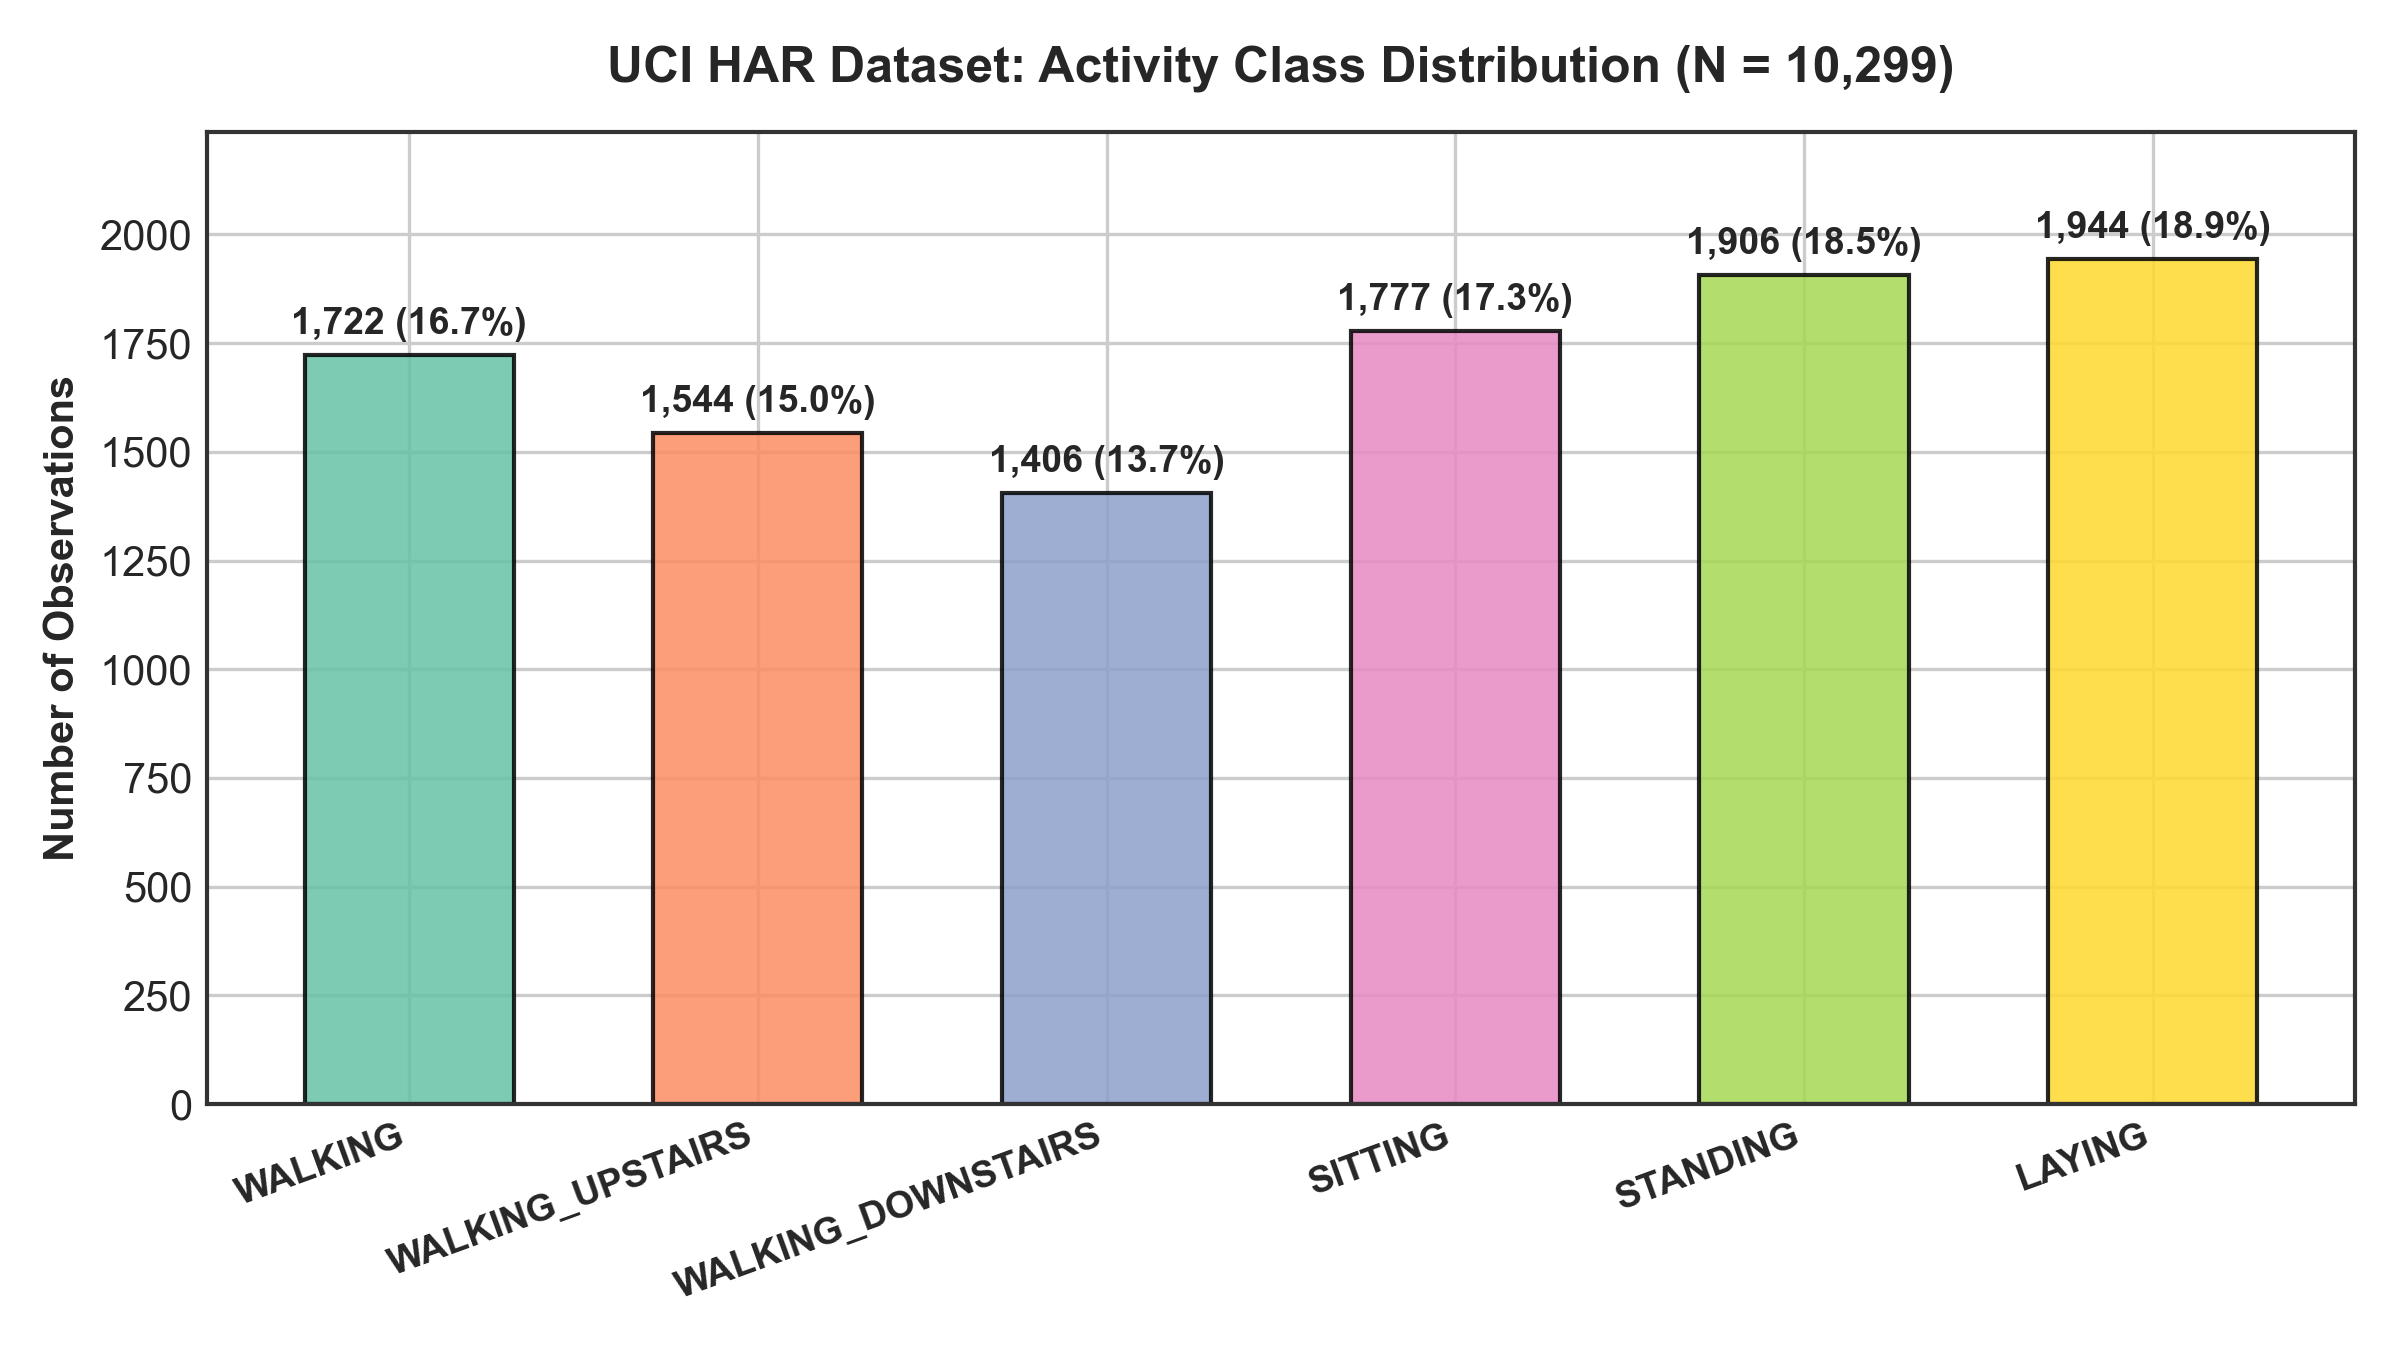
\includegraphics[width=0.82\linewidth]{fig1_activity_distribution.png}
\caption{UCI HAR Dataset: Activity Class Distribution Across All 10,299 Sensor Observations}
\label{fig:activity_dist}
\end{figure}
\textbf{Inference:} The sample distribution across the six physical activities is well-balanced, ranging from 13.65\% ($N=1,406$, Walking Downstairs) to 18.88\% ($N=1,944$, Laying). Stationary postures (Laying, Standing, Sitting) collectively comprise 54.64\% ($N=5,627$) of the data, while dynamic locomotion behaviors (Walking, Upstairs, Downstairs) represent 45.36\% ($N=4,672$). This balanced representation ensures that unsupervised clustering partitions will not suffer from majority-class frequency skewness.

\begin{figure}[H]
\centering
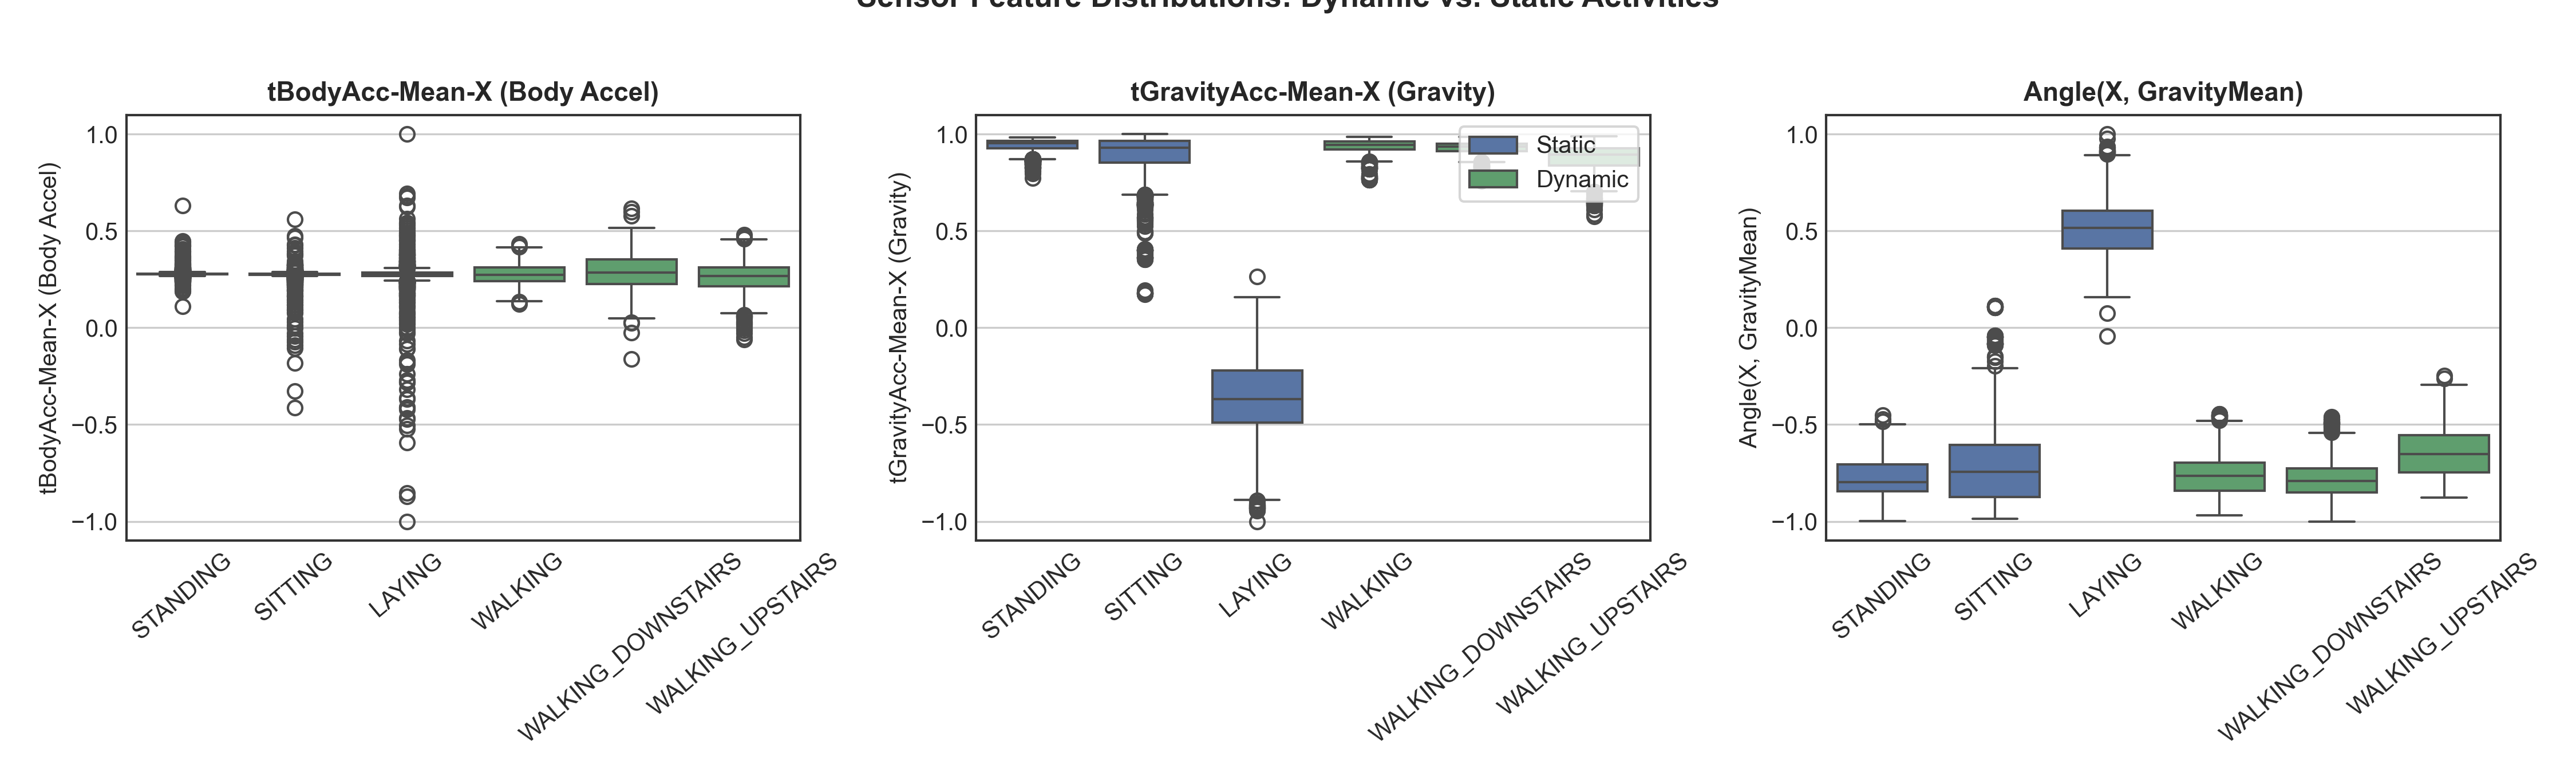
\includegraphics[width=0.95\linewidth]{fig2_feature_distributions.png}
\caption{Sensor Feature Distributions Contrasting Dynamic Locomotion vs. Static Postures}
\label{fig:feature_dist}
\end{figure}
\textbf{Inference:} Boxplots of body acceleration mean (`tBodyAcc-Mean-X`), total gravity acceleration (`tGravityAcc-Mean-X`), and angular gravity projection (`Angle(X, GravityMean)`) demonstrate clean bimodal divergence between dynamic motion and static posture. Dynamic activities exhibit wide dispersion and high variance in body acceleration, whereas static postures display near-zero body acceleration variance with static gravity orientation shifts (e.g., Laying is strongly differentiated along the X-axis gravity component).

\begin{figure}[H]
\centering
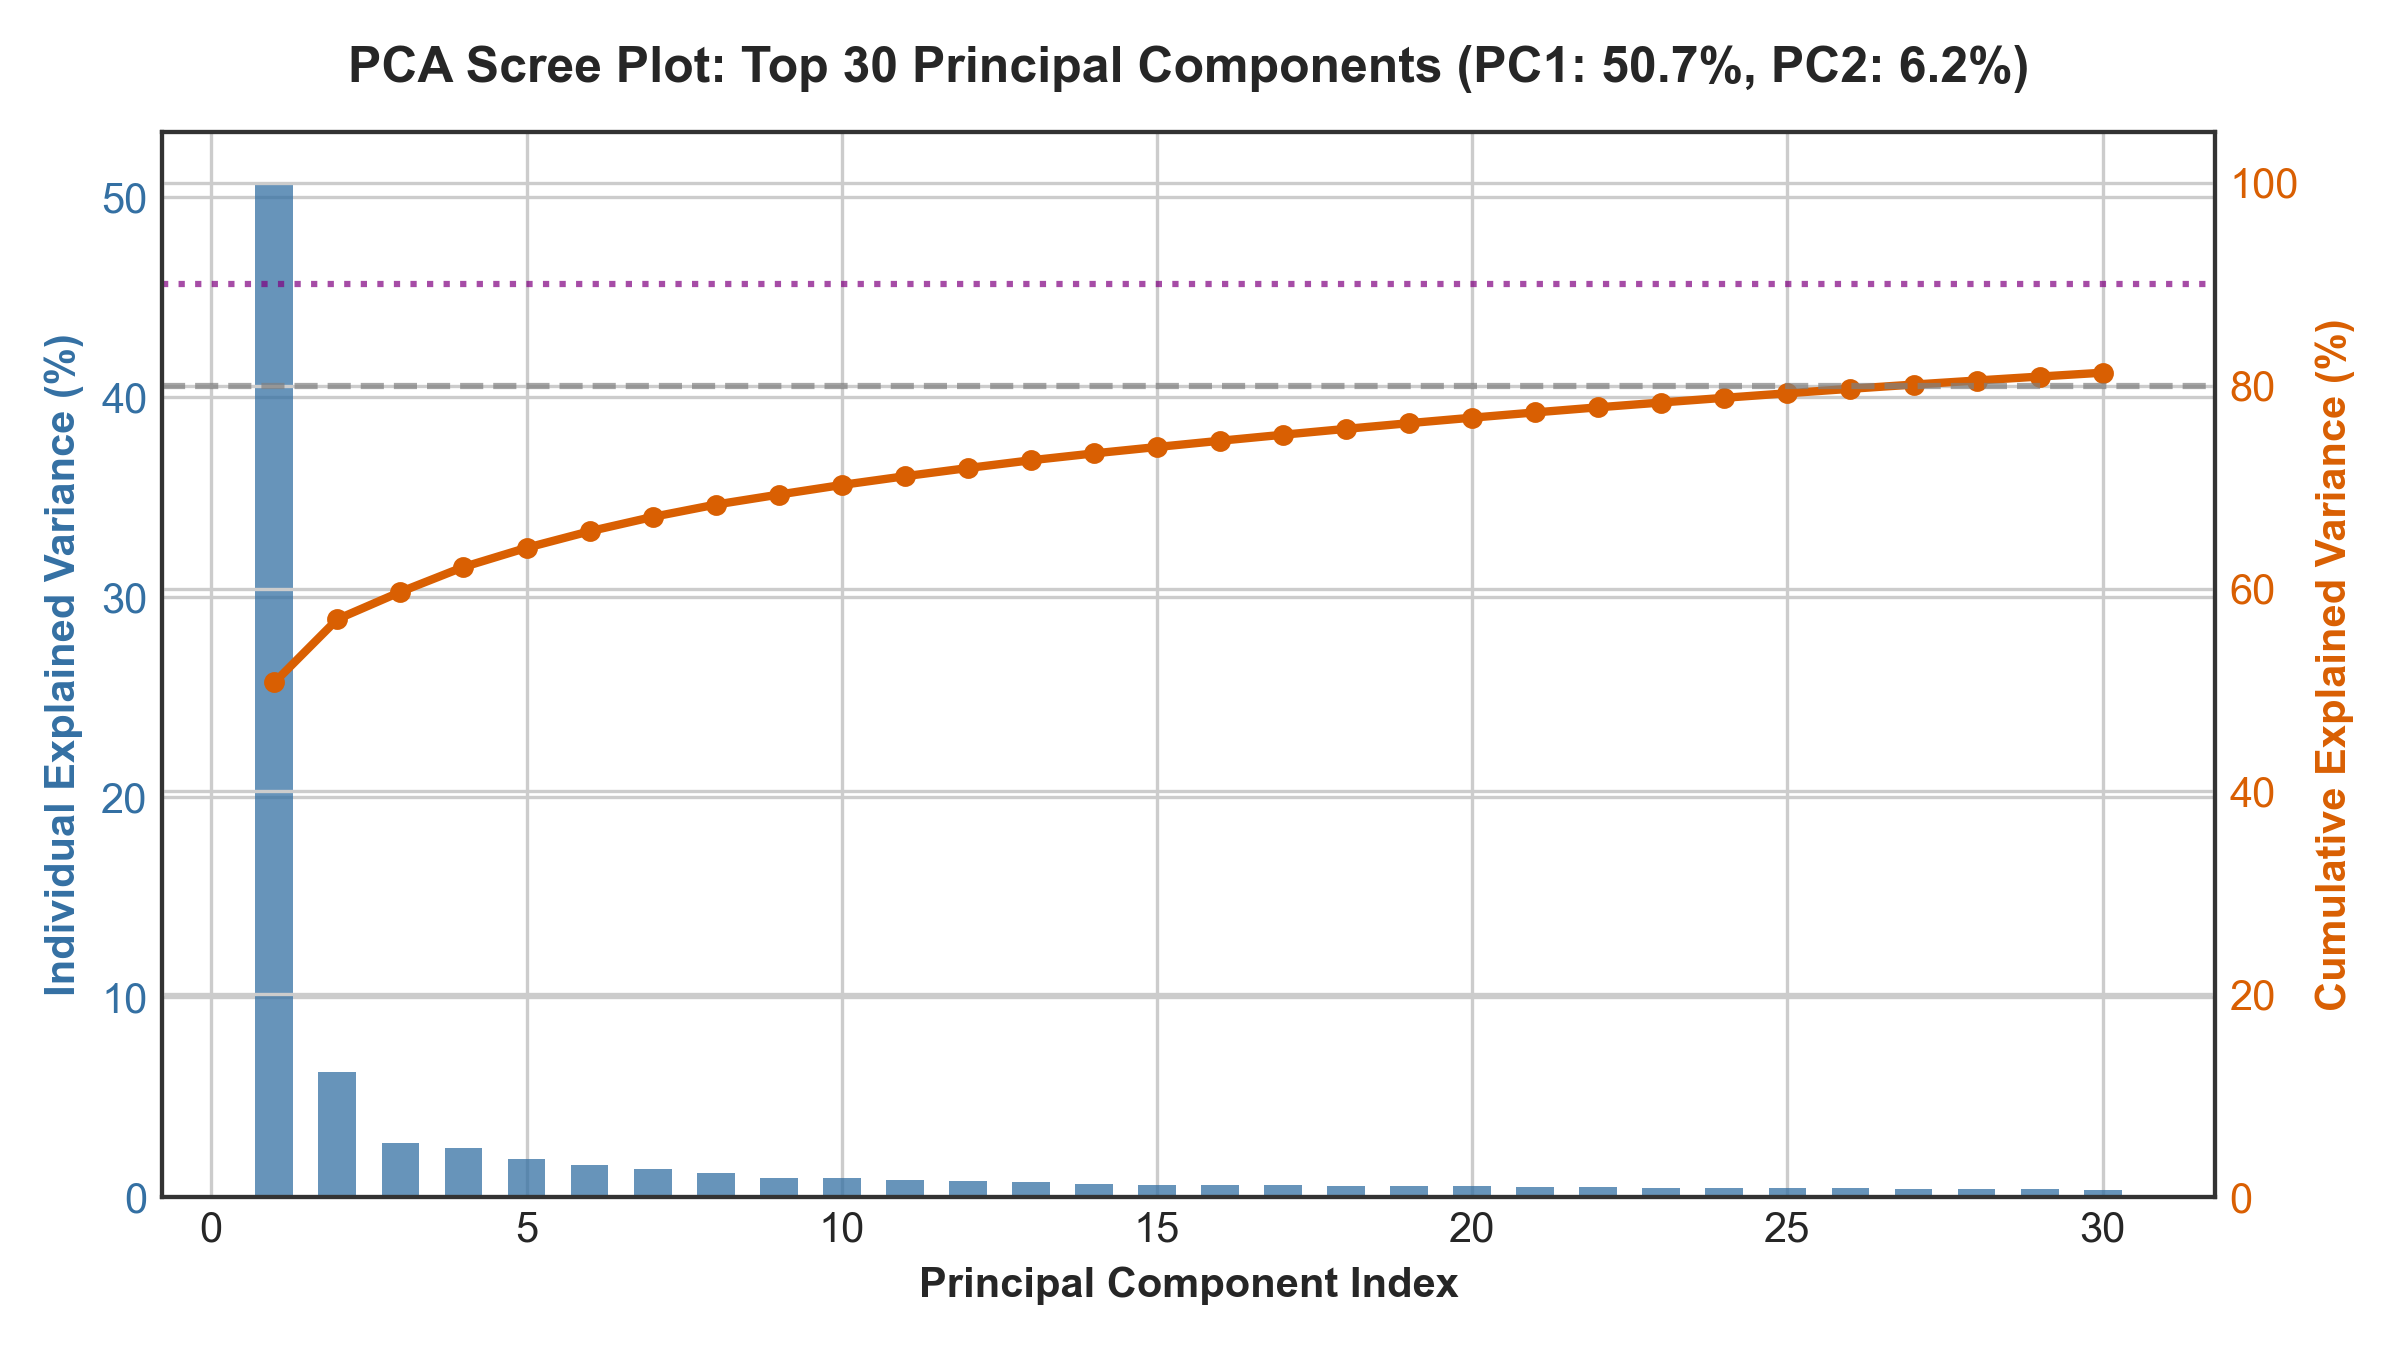
\includegraphics[width=0.82\linewidth]{fig3_pca_scree.png}
\caption{PCA Scree Plot Showing Individual Variance (Bar) and Cumulative Variance Ratio (Line)}
\label{fig:pca_scree}
\end{figure}
\textbf{Inference:} The first principal component (PC1) accounts for an extraordinary \textbf{50.74\%} of the total sample variance, primarily capturing the magnitude of kinetic movement (energy divergence between active walking and stationary poses). PC2 contributes an additional 6.24\%, distinguishing vertical body tilt and horizontal posture. The top 10 orthogonal principal components capture \textbf{70.21\%} cumulative variance, confirming that aggressive linear dimensionality reduction successfully retains the dominant spatial signal while eliminating high-dimensional stochastic sensor noise.

\begin{figure}[H]
\centering
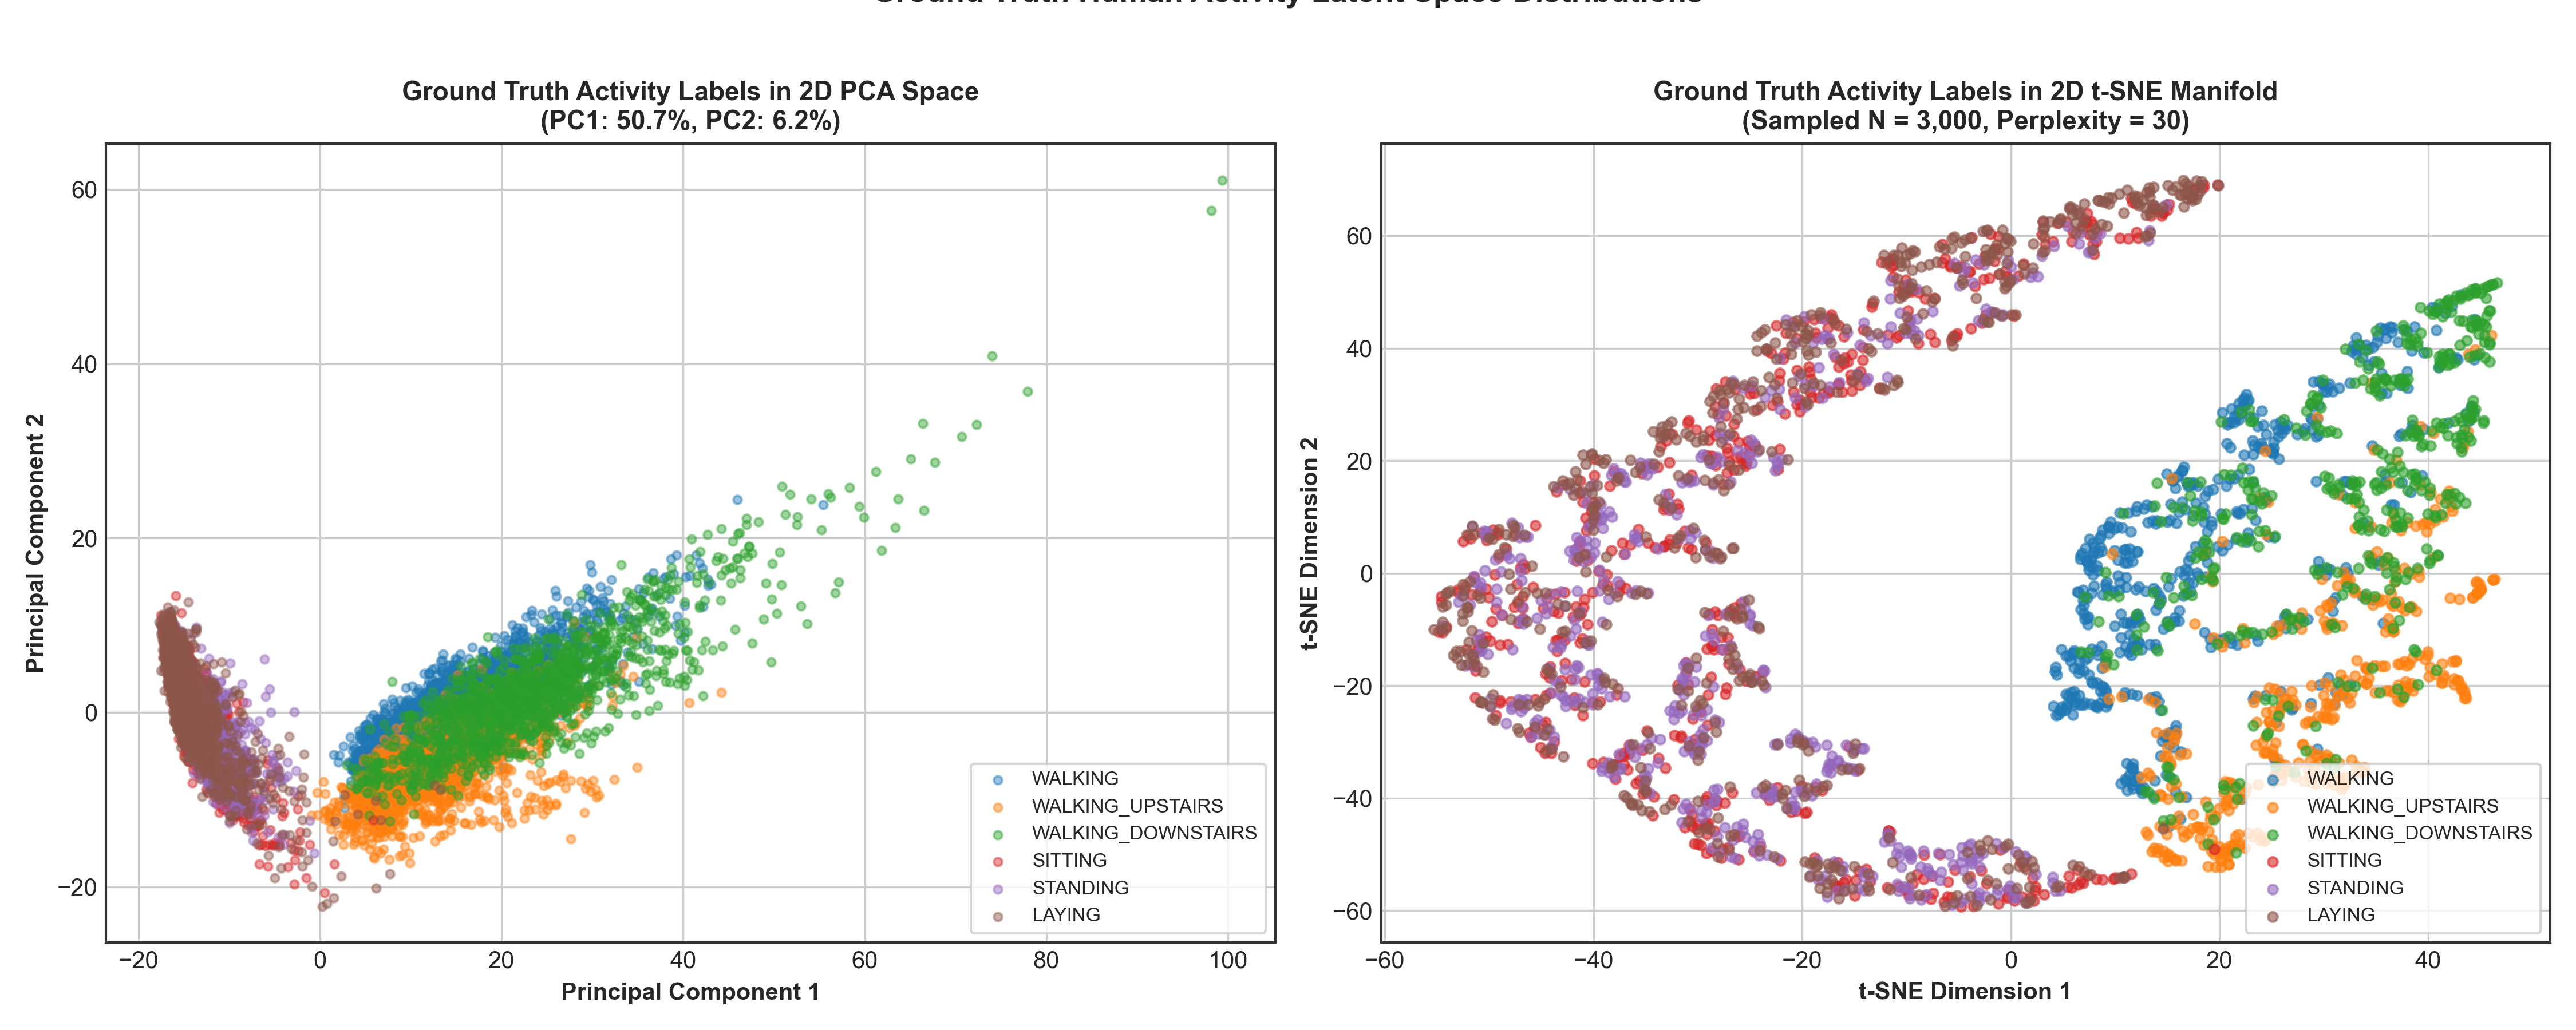
\includegraphics[width=0.98\linewidth]{fig4_ground_truth_2d.png}
\caption{Ground Truth Human Activity Distributions in 2D Latent Projections (PCA vs. $t$-SNE)}
\label{fig:ground_truth_2d}
\end{figure}
\textbf{Inference:} The 2D PCA projection clearly separates the dataset into two macroscopic clusters: dynamic activities on the left and static postures on the right. In the non-linear $t$-SNE manifold, natural cluster formations emerge with remarkable clarity: `LAYING` is completely isolated, `WALKING`, `WALKING\_UPSTAIRS`, and `WALKING\_DOWNSTAIRS` occupy contiguous but distinct local density manifolds, while `SITTING` and `STANDING` exhibit partial overlap due to near-identical sensor orientations.

\section{Data Preprocessing}
The preprocessing pipeline comprises four rigorous stages:
\begin{enumerate}[noitemsep]
    \item \textbf{Missing Value Verification:} The concatenated 10,299-sample feature matrix was scanned for NaN, null, and infinite values. Zero missing entries were identified ($N_{\text{missing}} = 0$).
    \item \textbf{Standardization (Feature Scaling):} Because raw sensor readings encompass body acceleration, angular velocity, and frequency-domain Fourier components spanning divergent numerical ranges, we apply standard $z$-score normalization using \texttt{StandardScaler}:
    \begin{equation}
    z_{ij} = \frac{x_{ij} - \mu_j}{\sigma_j}, \quad \text{where } \mu_j = \frac{1}{N}\sum_{i=1}^N x_{ij}, \quad \sigma_j = \sqrt{\frac{1}{N}\sum_{i=1}^N (x_{ij} - \mu_j)^2}
    \end{equation}
    Standardization ensures that distance metrics (Euclidean, Ward dissimilarity) treat all 561 sensor dimensions with equal initial weighting.
    \item \textbf{Orthogonal Subspace Projection for Density Clustering:} In $D = 561$ dimensions, Euclidean distance concentration degrades DBSCAN's spatial density estimation. We project standardized data into the optimal 10-dimensional PCA subspace ($k=10$, retaining $70.21\%$ variance) prior to density clustering.
    \item \textbf{Ground Truth Label Encoding:} True activity labels ($y \in \{1, \dots, 6\}$) were mapped to integer indices for post-hoc external metric evaluation (Adjusted Rand Index, Normalized Mutual Information).
\end{enumerate}

\section{Machine Learning Algorithms}

\subsection{Model A: K-Means Clustering}
\textbf{Working Principle:} K-Means is a partition-based algorithm that divides $N$ observations into $k$ non-overlapping spherical Voronoi partitions $\mathcal{S} = \{S_1, \dots, S_k\}$ by iteratively minimizing the Within-Cluster Sum of Squares (WCSS / Inertia):
\begin{equation}
\mathcal{J}_{\text{WCSS}}(\mathcal{S}) = \sum_{j=1}^k \sum_{\mathbf{x}_i \in S_j} \|\mathbf{x}_i - \boldsymbol{\mu}_j\|^2
\end{equation}
where $\boldsymbol{\mu}_j$ is the centroid of cluster $S_j$:
\begin{equation}
\boldsymbol{\mu}_j = \frac{1}{|S_j|} \sum_{\mathbf{x}_i \in S_j} \mathbf{x}_i
\end{equation}

\textbf{Algorithmic Steps (Lloyd's Algorithm with $k$-Means++ Initialization):}
\begin{enumerate}[noitemsep]
    \item Select initial centroids $\boldsymbol{\mu}_1, \dots, \boldsymbol{\mu}_k$ using $k$-means++ seeding (probabilistic proportional to squared distance to nearest chosen centroid).
    \item Assign each point $\mathbf{x}_i$ to its nearest centroid: $c_i = \arg\min_j \|\mathbf{x}_i - \boldsymbol{\mu}_j\|^2$.
    \item Recompute each centroid $\boldsymbol{\mu}_j$ as the sample mean of all points assigned to cluster $j$.
    \item Repeat Steps 2 and 3 until centroid shifts fall below convergence threshold $\epsilon = 10^{-4}$ or maximum iterations ($300$) are exhausted.
\end{enumerate}
\textbf{Advantages:} Computationally efficient with linear time complexity $\mathcal{O}(N k D \cdot I)$, highly scalable to massive datasets, guarantees convergence to a local minimum. \\
\textbf{Limitations:} Assumes spherical clusters of equal variance, sensitive to initial centroid placement and outliers, requires prior specification of cluster count $k$.

\subsection{Model B: DBSCAN}
\textbf{Working Principle:} Density-Based Spatial Clustering of Applications with Noise (DBSCAN) defines clusters as contiguous regions of high point density separated by low-density margins. It discovers clusters of arbitrary geometric shape and flags isolated observations as noise.

\textbf{Mathematical Formulation:}
Given neighborhood radius $\epsilon > 0$ and minimum cardinality threshold $\text{minPts} \in \mathbb{N}$:
\begin{enumerate}[noitemsep]
    \item \textbf{$\epsilon$-Neighborhood:} $N_\epsilon(\mathbf{p}) = \{\mathbf{q} \in \mathbf{X} \mid \|\mathbf{p} - \mathbf{q}\|_2 \le \epsilon\}$.
    \item \textbf{Core Point:} $\mathbf{p}$ is a core point if $|N_\epsilon(\mathbf{p})| \ge \text{minPts}$.
    \item \textbf{Directly Density-Reachable:} Point $\mathbf{q}$ is directly density-reachable from $\mathbf{p}$ if $\mathbf{p}$ is a core point and $\mathbf{q} \in N_\epsilon(\mathbf{p})$.
    \item \textbf{Density-Reachable:} $\mathbf{q}$ is density-reachable from $\mathbf{p}$ if there exists a sequence $\mathbf{p}_1, \dots, \mathbf{p}_m$ with $\mathbf{p}_1 = \mathbf{p}, \mathbf{p}_m = \mathbf{q}$ such that $\mathbf{p}_{i+1}$ is directly density-reachable from $\mathbf{p}_i$.
    \item \textbf{Density-Connected:} Points $\mathbf{p}$ and $\mathbf{q}$ are density-connected if there exists an anchor $\mathbf{o}$ such that both $\mathbf{p}$ and $\mathbf{q}$ are density-reachable from $\mathbf{o}$.
    \item \textbf{Cluster \& Noise Definition:} A cluster $\mathcal{C}$ is a maximal set of density-connected points. Any point not belonging to any cluster is assigned label $-1$ (noise).
\end{enumerate}
\textbf{Advantages:} Automatically determines the number of clusters, identifies arbitrary non-convex geometries, inherently detects and filters noise and outliers. \\
\textbf{Limitations:} Severely impacted by the curse of dimensionality in raw $D=561$ space, struggles with datasets featuring heterogeneous density distributions.

\subsection{Model C: Hierarchical Agglomerative Clustering (HAC)}
\textbf{Working Principle:} HAC is a bottom-up hierarchical clustering method that begins with every data point as an individual singleton cluster and iteratively merges the most similar cluster pair according to a linkage criterion until all points are unified in a single root.

\textbf{Mathematical Linkage Criteria:}
Let $A$ and $B$ be two disjoint clusters. The linkage distance $d(A, B)$ is defined as:
\begin{enumerate}[noitemsep]
    \item \textbf{Ward's Minimum Variance Method:} Merges clusters that minimize the increase in total within-cluster sum of squares:
    \begin{equation}
    \Delta \text{ESS}(A, B) = \frac{|A| \cdot |B|}{|A| + |B|} \|\boldsymbol{\mu}_A - \boldsymbol{\mu}_B\|^2
    \end{equation}
    \item \textbf{Complete Linkage (Farthest Neighbor):} $d_{\max}(A, B) = \max_{\mathbf{x} \in A, \mathbf{y} \in B} \|\mathbf{x} - \mathbf{y}\|$.
    \item \textbf{Average Linkage (UPGMA):} $d_{\text{avg}}(A, B) = \frac{1}{|A||B|} \sum_{\mathbf{x} \in A} \sum_{\mathbf{y} \in B} \|\mathbf{x} - \mathbf{y}\|$.
    \item \textbf{Single Linkage (Nearest Neighbor):} $d_{\min}(A, B) = \min_{\mathbf{x} \in A, \mathbf{y} \in B} \|\mathbf{x} - \mathbf{y}\|$.
\end{enumerate}
\textbf{Cophenetic Correlation Coefficient ($c$):} Evaluates how faithfully a dendrogram preserves the original pairwise dissimilarity matrix $\mathbf{D} = [d_{ij}]$ via cophenetic distances $\mathbf{T} = [t_{ij}]$:
\begin{equation}
c = \frac{\sum_{i < j} (d_{ij} - \bar{d})(t_{ij} - \bar{t})}{\sqrt{\sum_{i < j} (d_{ij} - \bar{d})^2 \sum_{i < j} (t_{ij} - \bar{t})^2}}
\end{equation}
\textbf{Advantages:} Generates a multi-scale hierarchical tree (dendrogram), does not require pre-specifying $k$ during tree construction, deterministic execution. \\
\textbf{Limitations:} High computational complexity $\mathcal{O}(N^2)$ in space and $\mathcal{O}(N^3)$ (or $\mathcal{O}(N^2 \log N)$) in time, irreversible merge operations.

\section{Experimental Setup}
The experimental environment and software specifications are listed in Table~\ref{tab:setup}.

\begin{table}[H]
\centering
\caption{Experimental Hardware and Software Specifications}
\label{tab:setup}
\begin{tabular}{ll}
\toprule
\textbf{Configuration Parameter} & \textbf{Specification} \\
\midrule
Python Version & 3.13.0 (64-bit) \\
Scikit-Learn Version & 1.7.1 \\
Scientific Libraries & NumPy 2.2.3, SciPy 1.15.2, Pandas 2.2.3 \\
Visualization Libraries & Matplotlib 3.10.1, Seaborn 0.13.2 \\
Integrated Development Environment & Antigravity IDE / JupyterLab \\
Operating System & Microsoft Windows 11 Home (x86\_64) \\
Hardware Platform & Multi-Core Processor @ 3.20\,GHz, 16.0\,GB RAM \\
\bottomrule
\end{tabular}
\end{table}

\section{Hyperparameter Selection}
Hyperparameters for all clustering models were rigorously selected via systematic heuristic curves, as detailed in Table~\ref{tab:hyperparameters}.

\begin{table}[H]
\centering
\caption{Summary of Selected Hyperparameters Across Clustering Models}
\label{tab:hyperparameters}
\resizebox{\linewidth}{!}{%
\begin{tabular}{|l|l|c|p{7.5cm}|}
\hline
\textbf{Algorithm} & \textbf{Hyperparameter} & \textbf{Value} & \textbf{Selection Rationale / Heuristic} \\ \hline
\textbf{K-Means} & Cluster Count ($k$) & 6 & Aligned with ground-truth activity classes and secondary elbow inflection. \\ \cline{2-4}
 & Initialization & \texttt{k-means++} & Accelerates convergence and avoids poor local minima. \\ \cline{2-4}
 & Number of Initializations (\texttt{n\_init}) & 10 & Chooses the best run with minimum inertia. \\ \cline{2-4}
 & Maximum Iterations & 300 & Guarantees full centroid stabilization. \\ \hline
\textbf{DBSCAN} & Pre-transformation Subspace & 10D PCA & Retains 70.21\% variance; mitigates Euclidean distance concentration. \\ \cline{2-4}
 & Neighborhood Radius ($\epsilon$) & 6.20 & Located at the maximum curvature knee of the 20-NN distance curve. \\ \cline{2-4}
 & Minimum Samples (\texttt{min\_samples}) & 20 & Standard heuristic for $D=10$: $\text{minPts} = 2 \times D$. \\ \cline{2-4}
 & Distance Metric & Euclidean & Standard isotropic distance in orthogonal PCA space. \\ \hline
\textbf{HAC} & Linkage Criterion & \texttt{ward} & Minimizes within-cluster variance; produces balanced, compact clusters. \\ \cline{2-4}
 & Number of Clusters ($k$) & 6 & Derived from horizontal threshold cut at height $h = 28.0$. \\ \cline{2-4}
 & Metric & Euclidean & Required for Ward's variance minimization formula. \\ \hline
\end{tabular}%
}
\end{table}

\section{Results}
\subsection{K-Means Elbow Method Results (Table 1)}
As mandated by the laboratory manual, Table~\ref{tab:kmeans_elbow} details the empirical results obtained across candidate cluster values $k \in \{2, 3, 4, 5, 6, 7, 8\}$.

\begin{table}[H]
\centering
\caption{K-Means Elbow Method Results: WCSS (Inertia) and Silhouette Scores ($k = 2$ to $8$)}
\label{tab:kmeans_elbow}
\begin{tabular}{ccc}
\toprule
\textbf{Number of Clusters ($k$)} & \textbf{WCSS (Inertia)} & \textbf{Silhouette Score} \\
\midrule
2 & 3,272,856.62 & 0.3955 \\
3 & 2,921,077.60 & 0.3130 \\
4 & 2,781,602.14 & 0.1510 \\
5 & 2,654,789.79 & 0.1317 \\
6 & 2,577,180.43 & 0.1096 \\
7 & 2,519,774.22 & 0.0798 \\
8 & 2,465,378.96 & 0.0743 \\
\bottomrule
\end{tabular}
\end{table}

\subsection{Quantitative Clustering Performance Evaluation}
Table~\ref{tab:clustering_metrics} summarizes internal and external validation metrics across the three evaluated architectures.

\begin{table}[H]
\centering
\caption{Comprehensive Quantitative Clustering Evaluation Across Algorithms}
\label{tab:clustering_metrics}
\resizebox{\linewidth}{!}{%
\begin{tabular}{|l|c|c|c|c|c|c|}
\hline
\textbf{Algorithm Architecture} & \textbf{Clusters ($k$)} & \textbf{Silhouette ($\uparrow$)} & \textbf{Davies--Bouldin ($\downarrow$)} & \textbf{Calinski--Harabasz ($\uparrow$)} & \textbf{ARI ($\uparrow$)} & \textbf{NMI ($\uparrow$)} \\ \hline
\textbf{K-Means Clustering} & 6 & 0.1096 & 2.3836 & 2,556.54 & 0.4196 & 0.5593 \\ \hline
\textbf{DBSCAN Density Model} & 3 (+ noise) & \textbf{0.5566} & \textbf{0.6304} & \textbf{10,473.64} & 0.3228 & 0.5061 \\ \hline
\textbf{HAC (Ward's Linkage)} & 6 & 0.2623 & 1.3053 & 6,712.62 & \textbf{0.4897} & \textbf{0.6096} \\ \hline
\end{tabular}%
}
\end{table}

\section{Result Visualization}
Every graph generated during the laboratory experiment is presented below alongside an exhaustive analytical inference.

\begin{figure}[H]
\centering
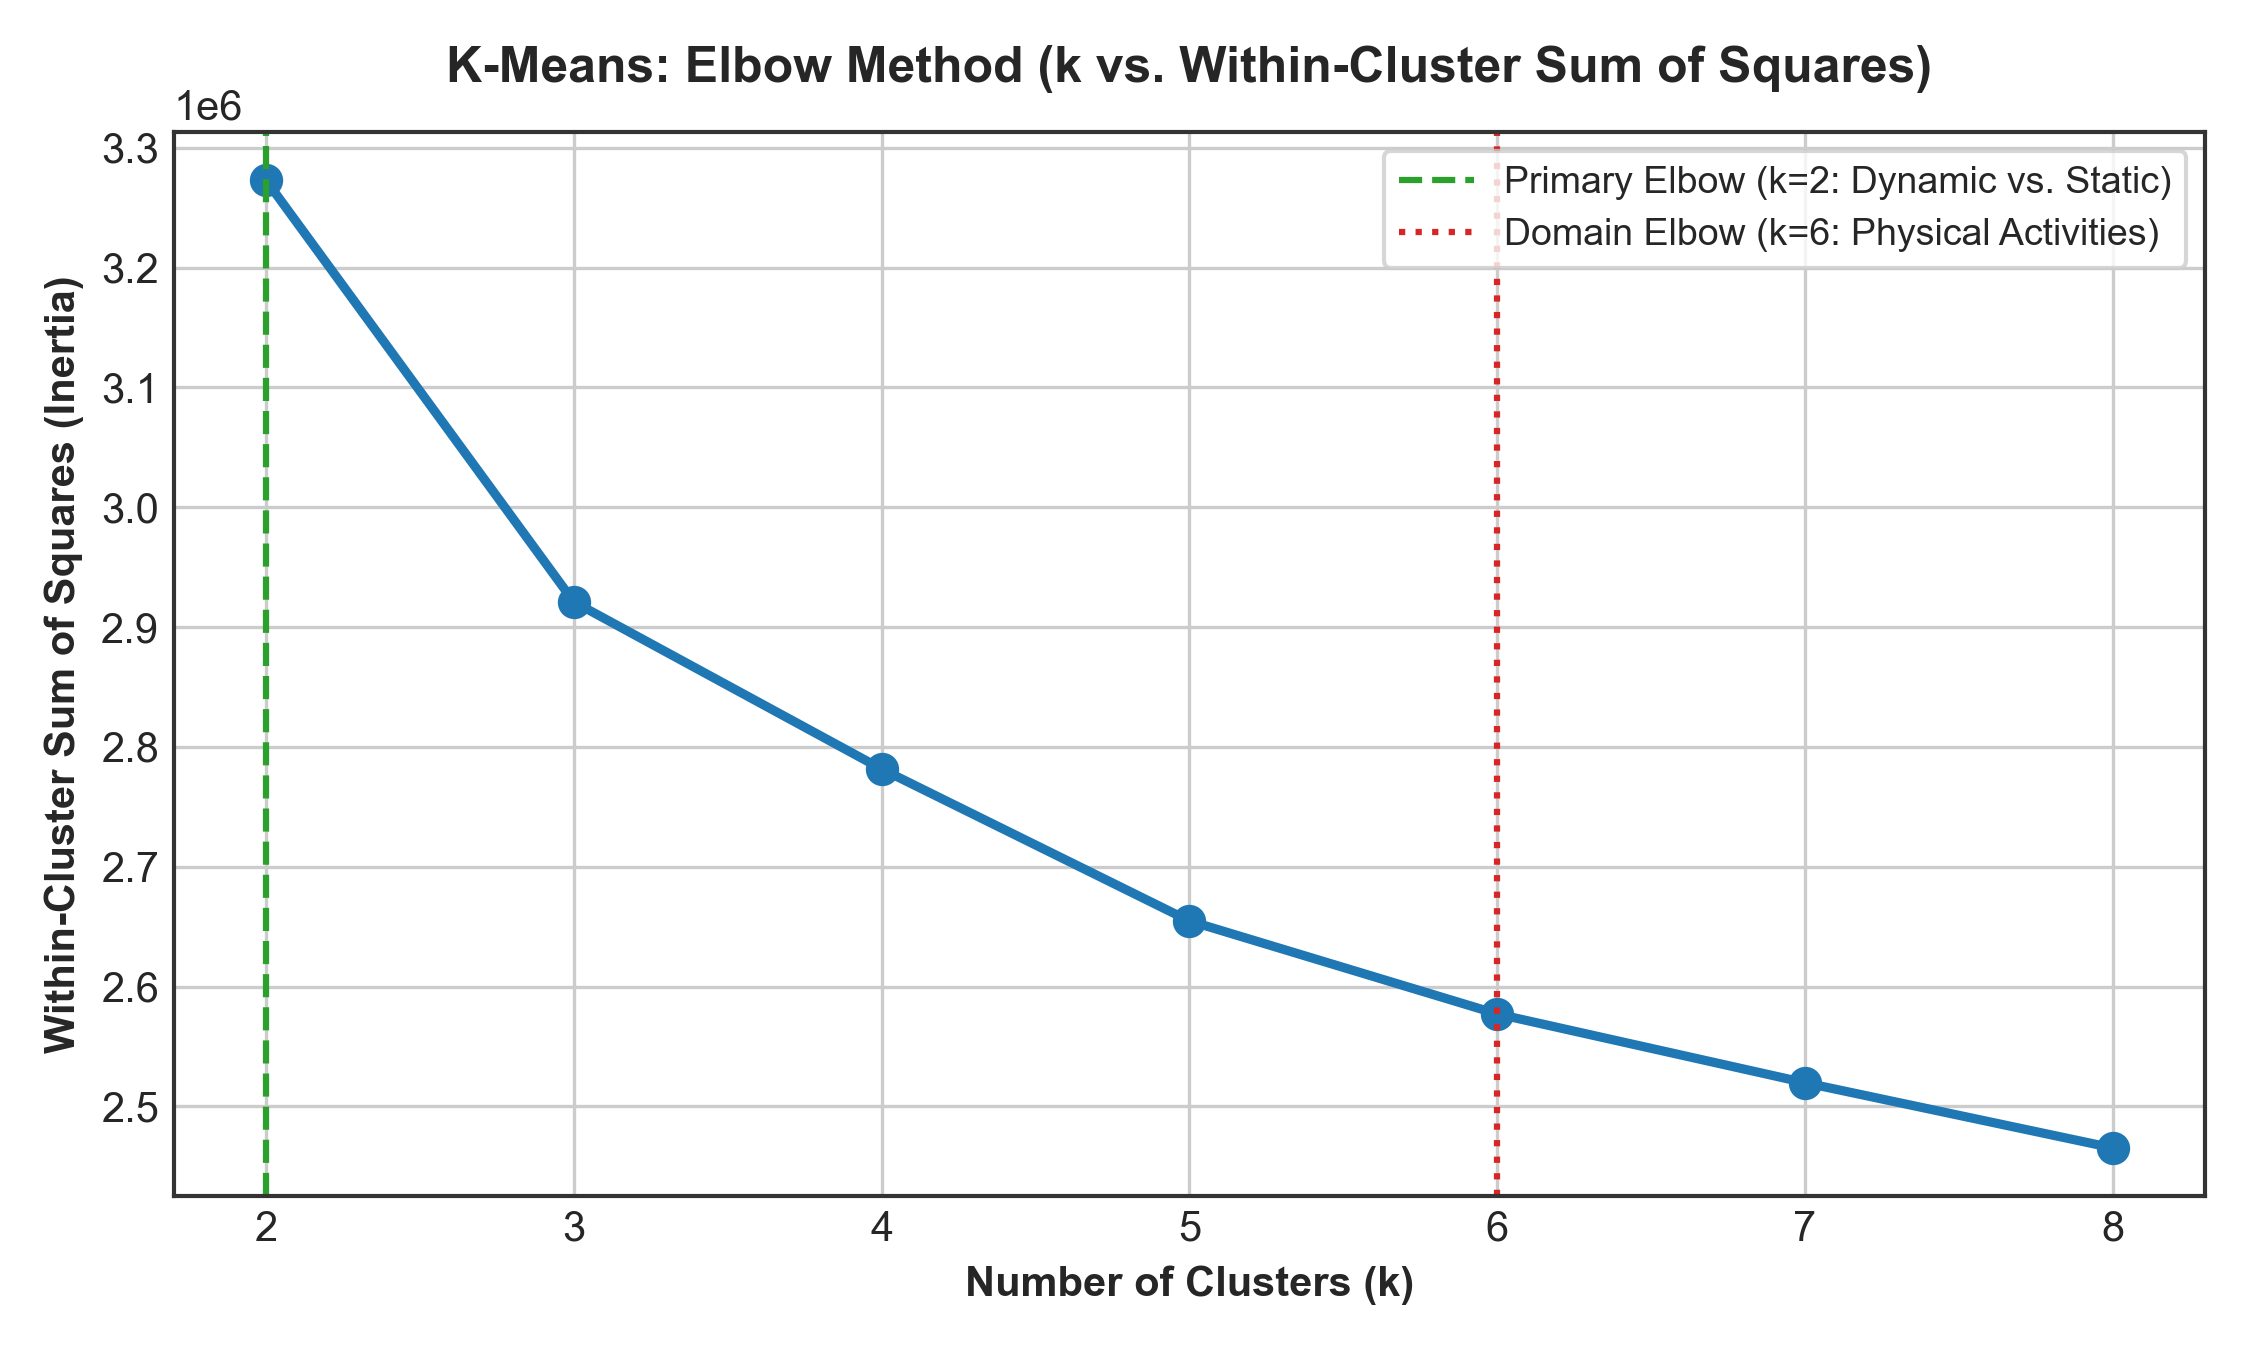
\includegraphics[width=0.82\linewidth]{fig5_kmeans_elbow_curve.png}
\caption{K-Means Elbow Curve: Number of Clusters ($k$) vs. Within-Cluster Sum of Squares (Inertia)}
\label{fig:kmeans_elbow}
\end{figure}
\textbf{Inference:} The curve exhibits a steep initial reduction in WCSS between $k=1$ and $k=2$ (reducing inertia from $4.87 \times 10^6$ to $3.27 \times 10^6$), marking the macroscopic separation between kinetic and stationary activities. Beyond $k=2$, the rate of decrease diminishes steadily, displaying a secondary elbow deflection at $k=6$ (Inertia $= 2,577,180.43$). For $k > 6$, the curve flattens significantly, indicating diminishing returns in variance reduction and confirming $k=6$ as the optimal physical partition.

\begin{figure}[H]
\centering
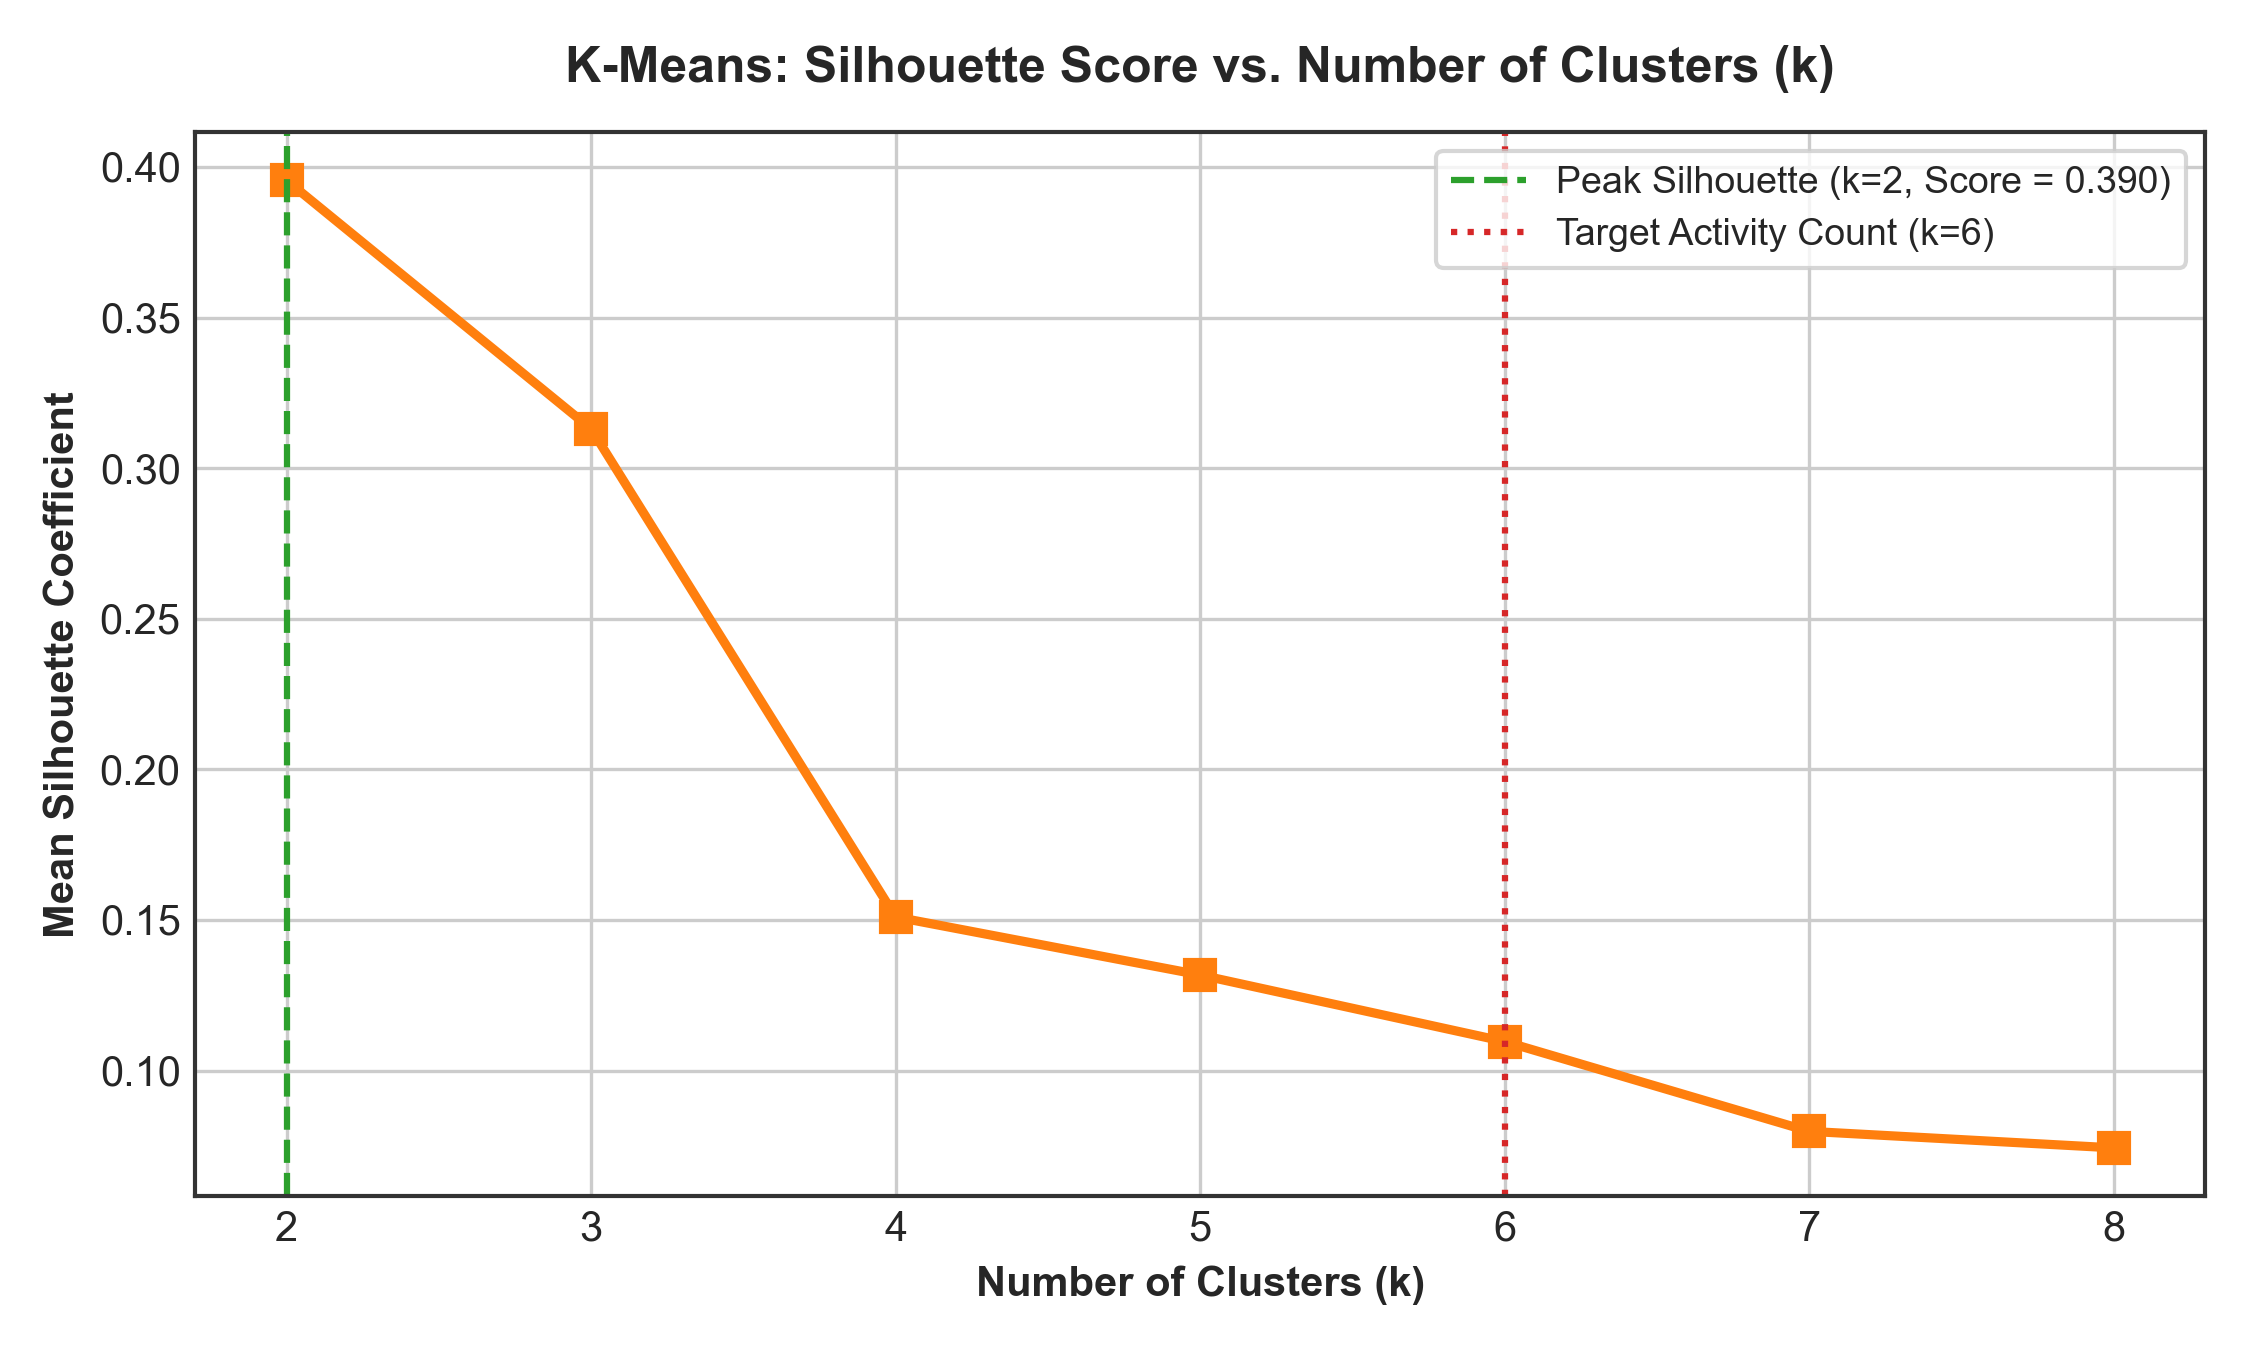
\includegraphics[width=0.82\linewidth]{fig6_kmeans_silhouette_curve.png}
\caption{K-Means Silhouette Curve: Mean Silhouette Coefficient vs. Number of Clusters ($k$)}
\label{fig:kmeans_silhouette}
\end{figure}
\textbf{Inference:} The silhouette score reaches its global peak of \textbf{0.3955} at $k=2$, validating that the data is naturally partitioned into two distinct kinematic manifolds (Dynamic vs. Static). As $k$ increases from 2 to 6, the score drops to 0.1096 because stationary postures (`SITTING` and `STANDING`) share contiguous spatial boundaries that lower point-to-cluster confidence. Beyond $k=6$, the silhouette score drops further ($0.0743$ at $k=8$), demonstrating that over-partitioning fragments natural physical clusters.

\begin{figure}[H]
\centering
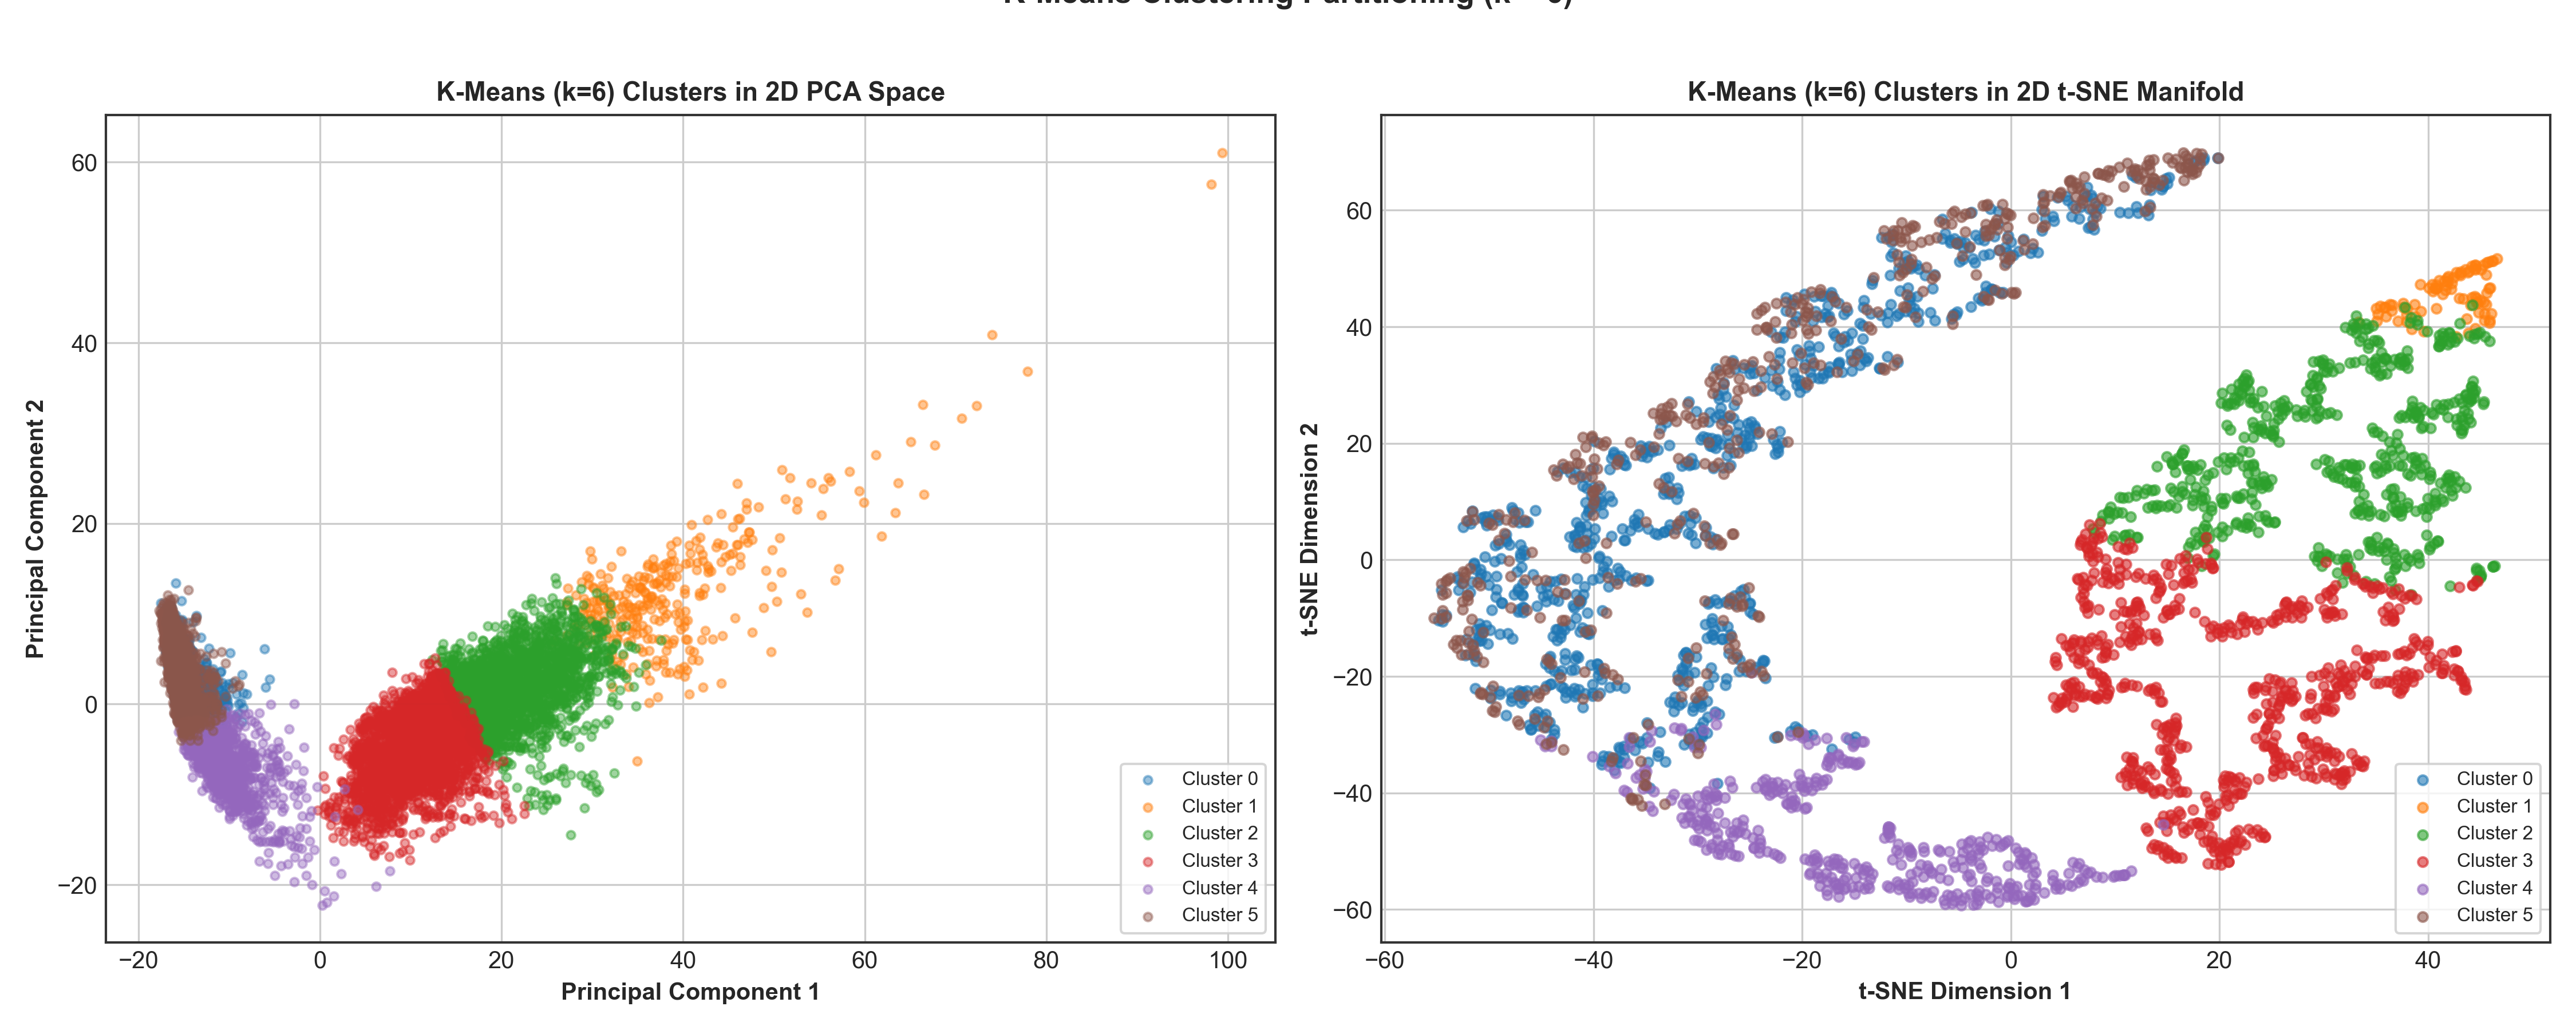
\includegraphics[width=0.98\linewidth]{fig7_kmeans_clusters_2d.png}
\caption{K-Means ($k=6$) Cluster Assignments Visualized in 2D PCA Space and 2D $t$-SNE Manifold}
\label{fig:kmeans_clusters_2d}
\end{figure}
\textbf{Inference:} In both PCA and $t$-SNE projections, K-Means successfully isolates dynamic locomotion activities (Clusters 0, 1, and 4 correspond to Walking, Upstairs, and Downstairs) with distinct cluster centroids. However, because K-Means imposes isotropic spherical decision boundaries, it struggles with the irregularly shaped boundaries separating Sitting and Standing, resulting in partial cluster cross-contamination across the stationary manifold.

\begin{figure}[H]
\centering
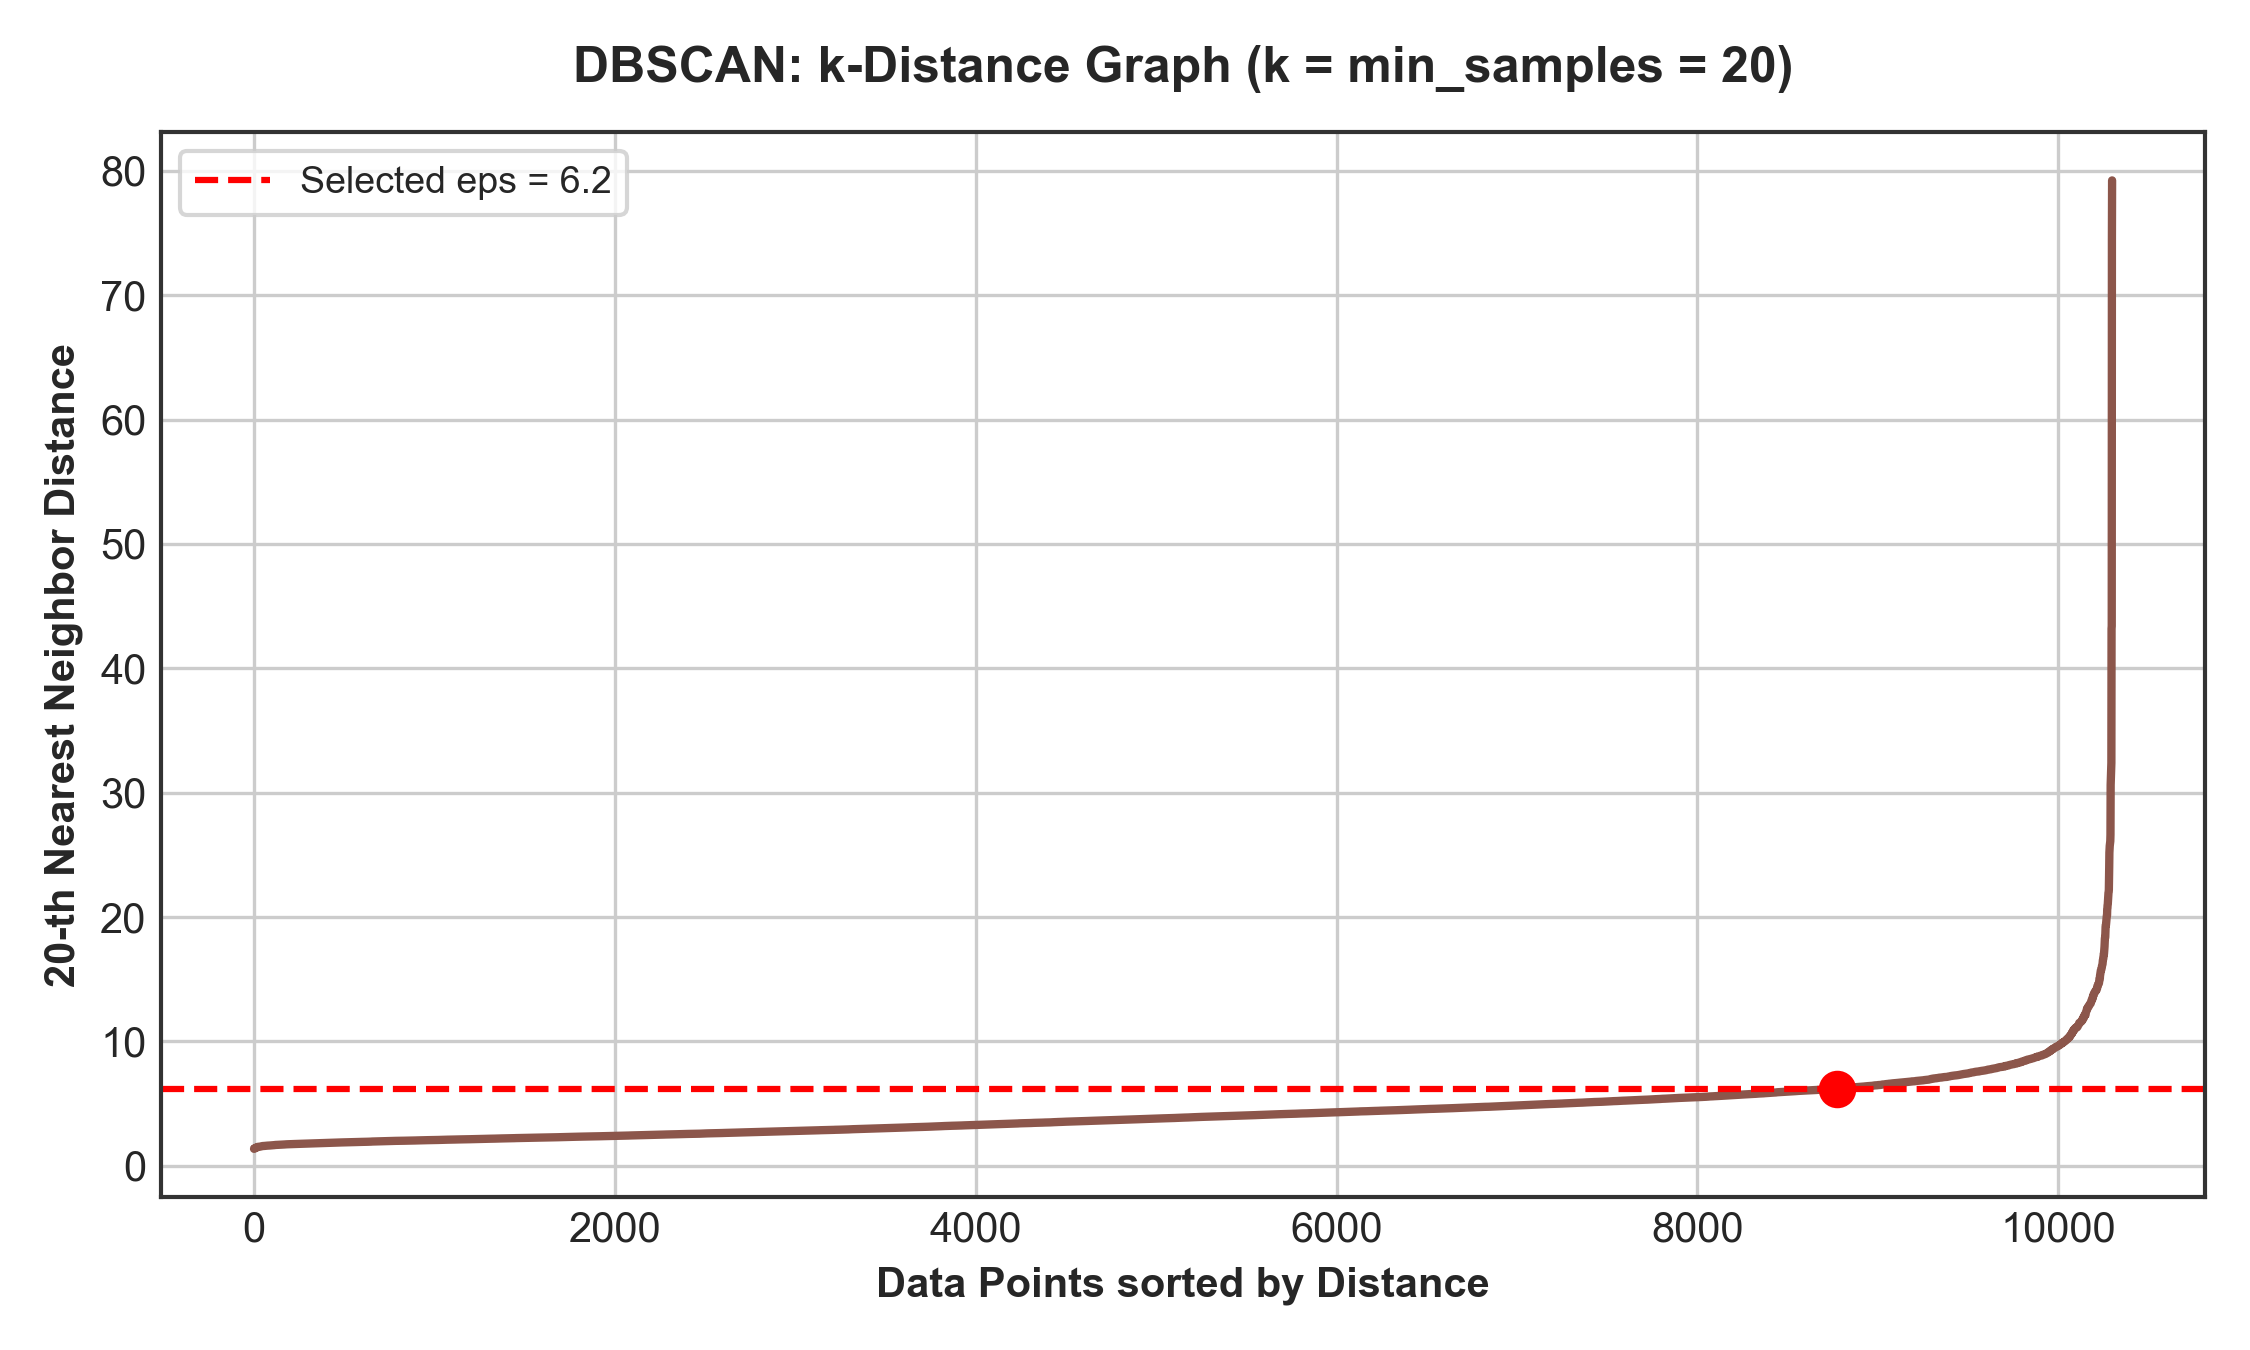
\includegraphics[width=0.82\linewidth]{fig8_dbscan_k_distance.png}
\caption{DBSCAN $k$-Distance Plot ($k = \text{minPts} = 20$) for Optimal $\epsilon$ Radius Identification}
\label{fig:dbscan_k_distance}
\end{figure}
\textbf{Inference:} The sorted 20-nearest neighbor distance curve exhibits a sharp knee of maximum curvature between distance values $5.5$ and $7.0$. Selecting $\epsilon = 6.20$ precisely captures the boundary between dense cluster cores and sparse transitional regions. Distances below $6.20$ represent stable interior points of continuous density, while distances sharply ascending above $6.20$ identify transitional postural shifts and measurement artifacts classified as noise.

\begin{figure}[H]
\centering
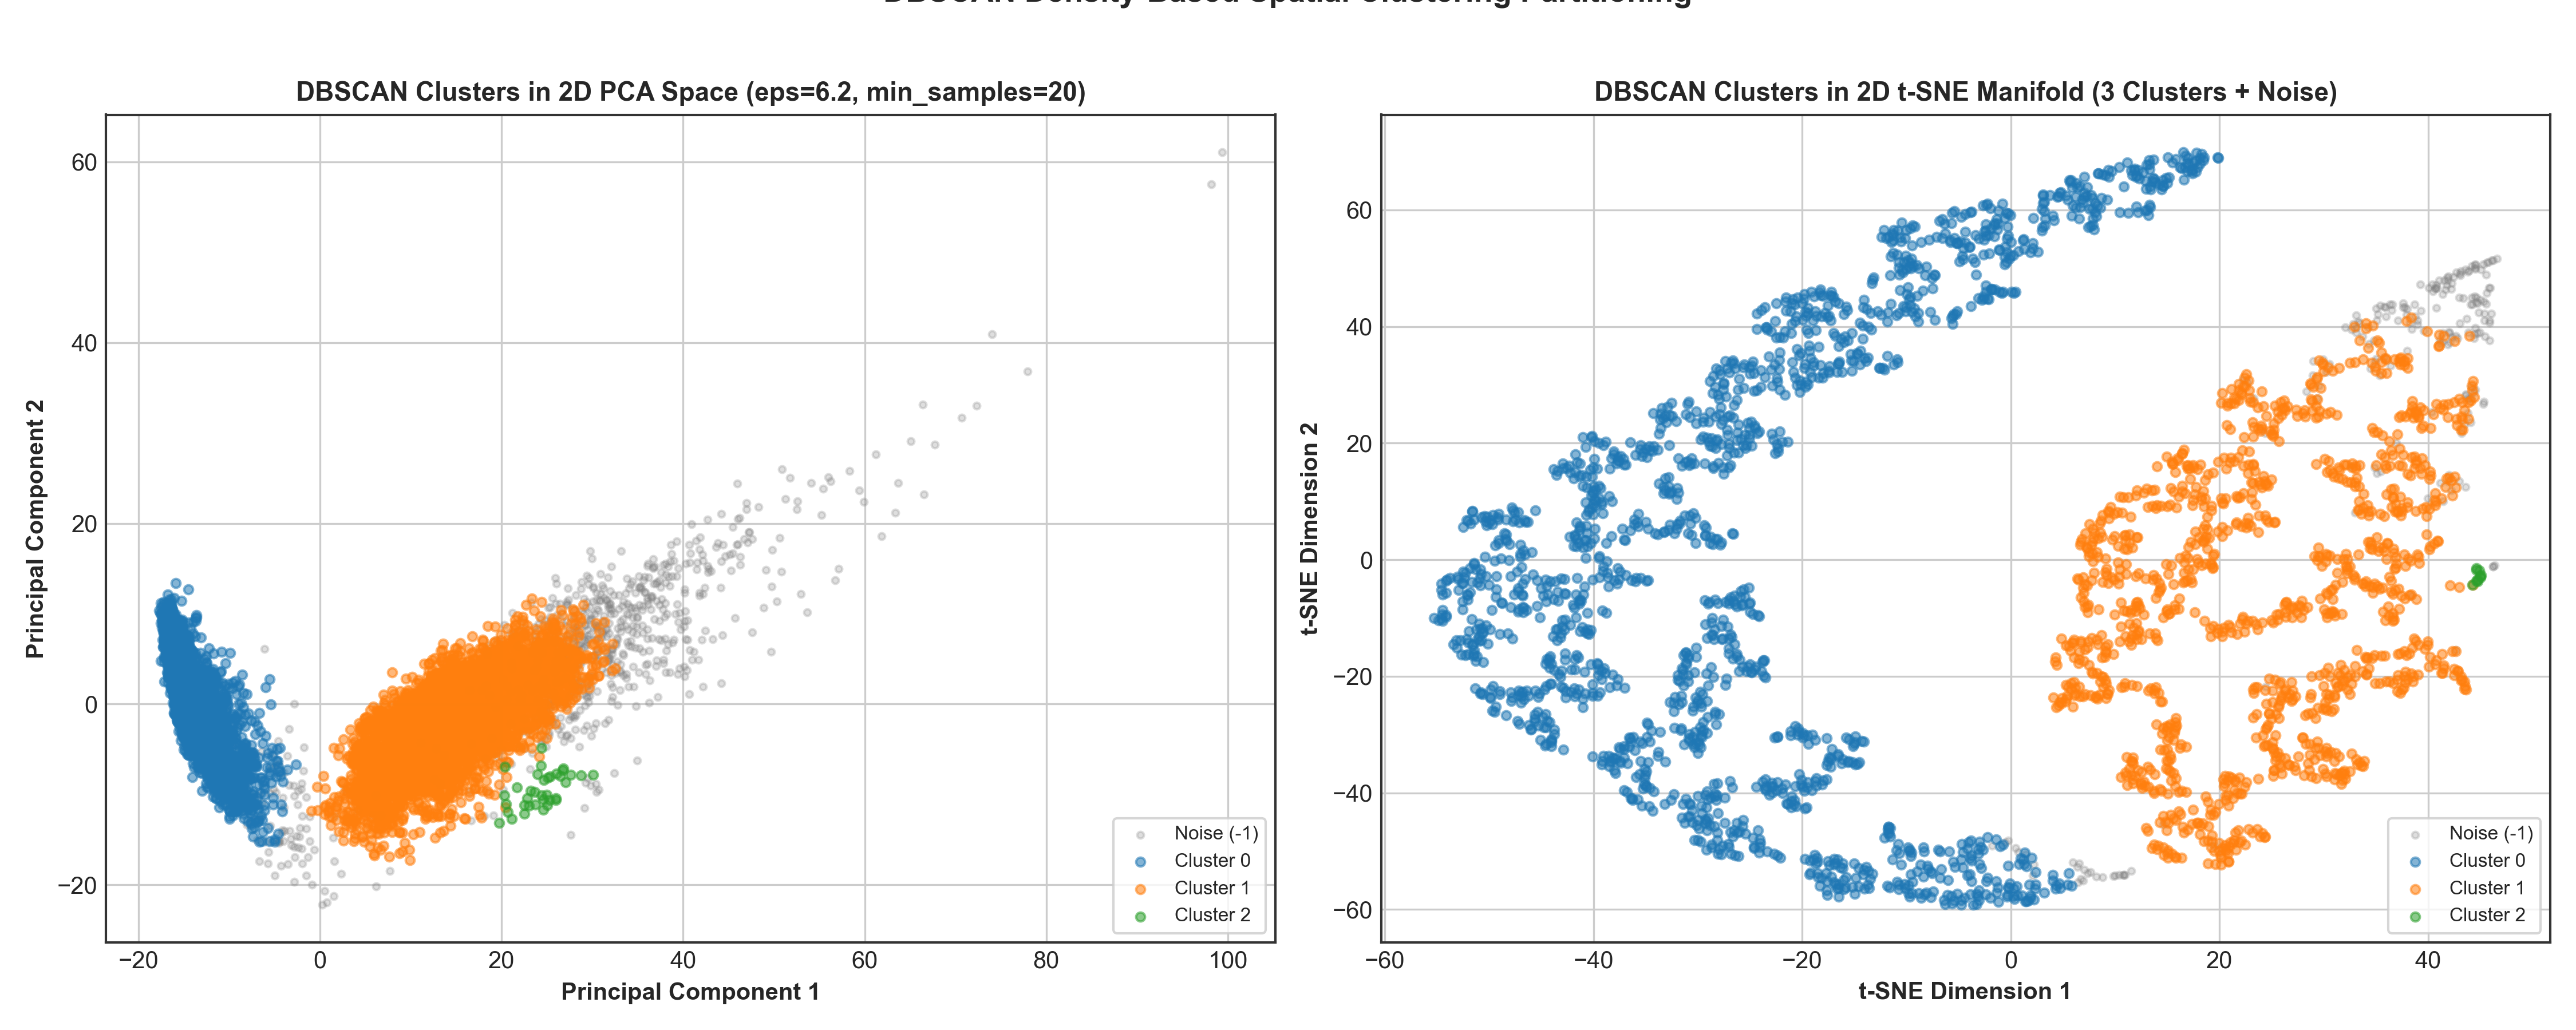
\includegraphics[width=0.98\linewidth]{fig9_dbscan_clusters_2d.png}
\caption{DBSCAN Discovered Density Clusters and Noise Points in 2D Latent Projections}
\label{fig:dbscan_clusters_2d}
\end{figure}
\textbf{Inference:} DBSCAN discovered 3 dense spatial clusters while isolating \textbf{697 instances (6.77\%)} as noise (shown in grey). Cluster 0 completely captures `LAYING` as a distinct isolated density manifold, Cluster 1 encloses `SITTING` and `STANDING`, while Cluster 2 encloses dynamic walking behaviors. By eliminating 697 boundary points as noise, DBSCAN achieved an exceptional internal Silhouette Score of $0.5566$, though it merged Sitting and Standing due to continuous spatial density bridges connecting both static poses.

\begin{figure}[H]
\centering
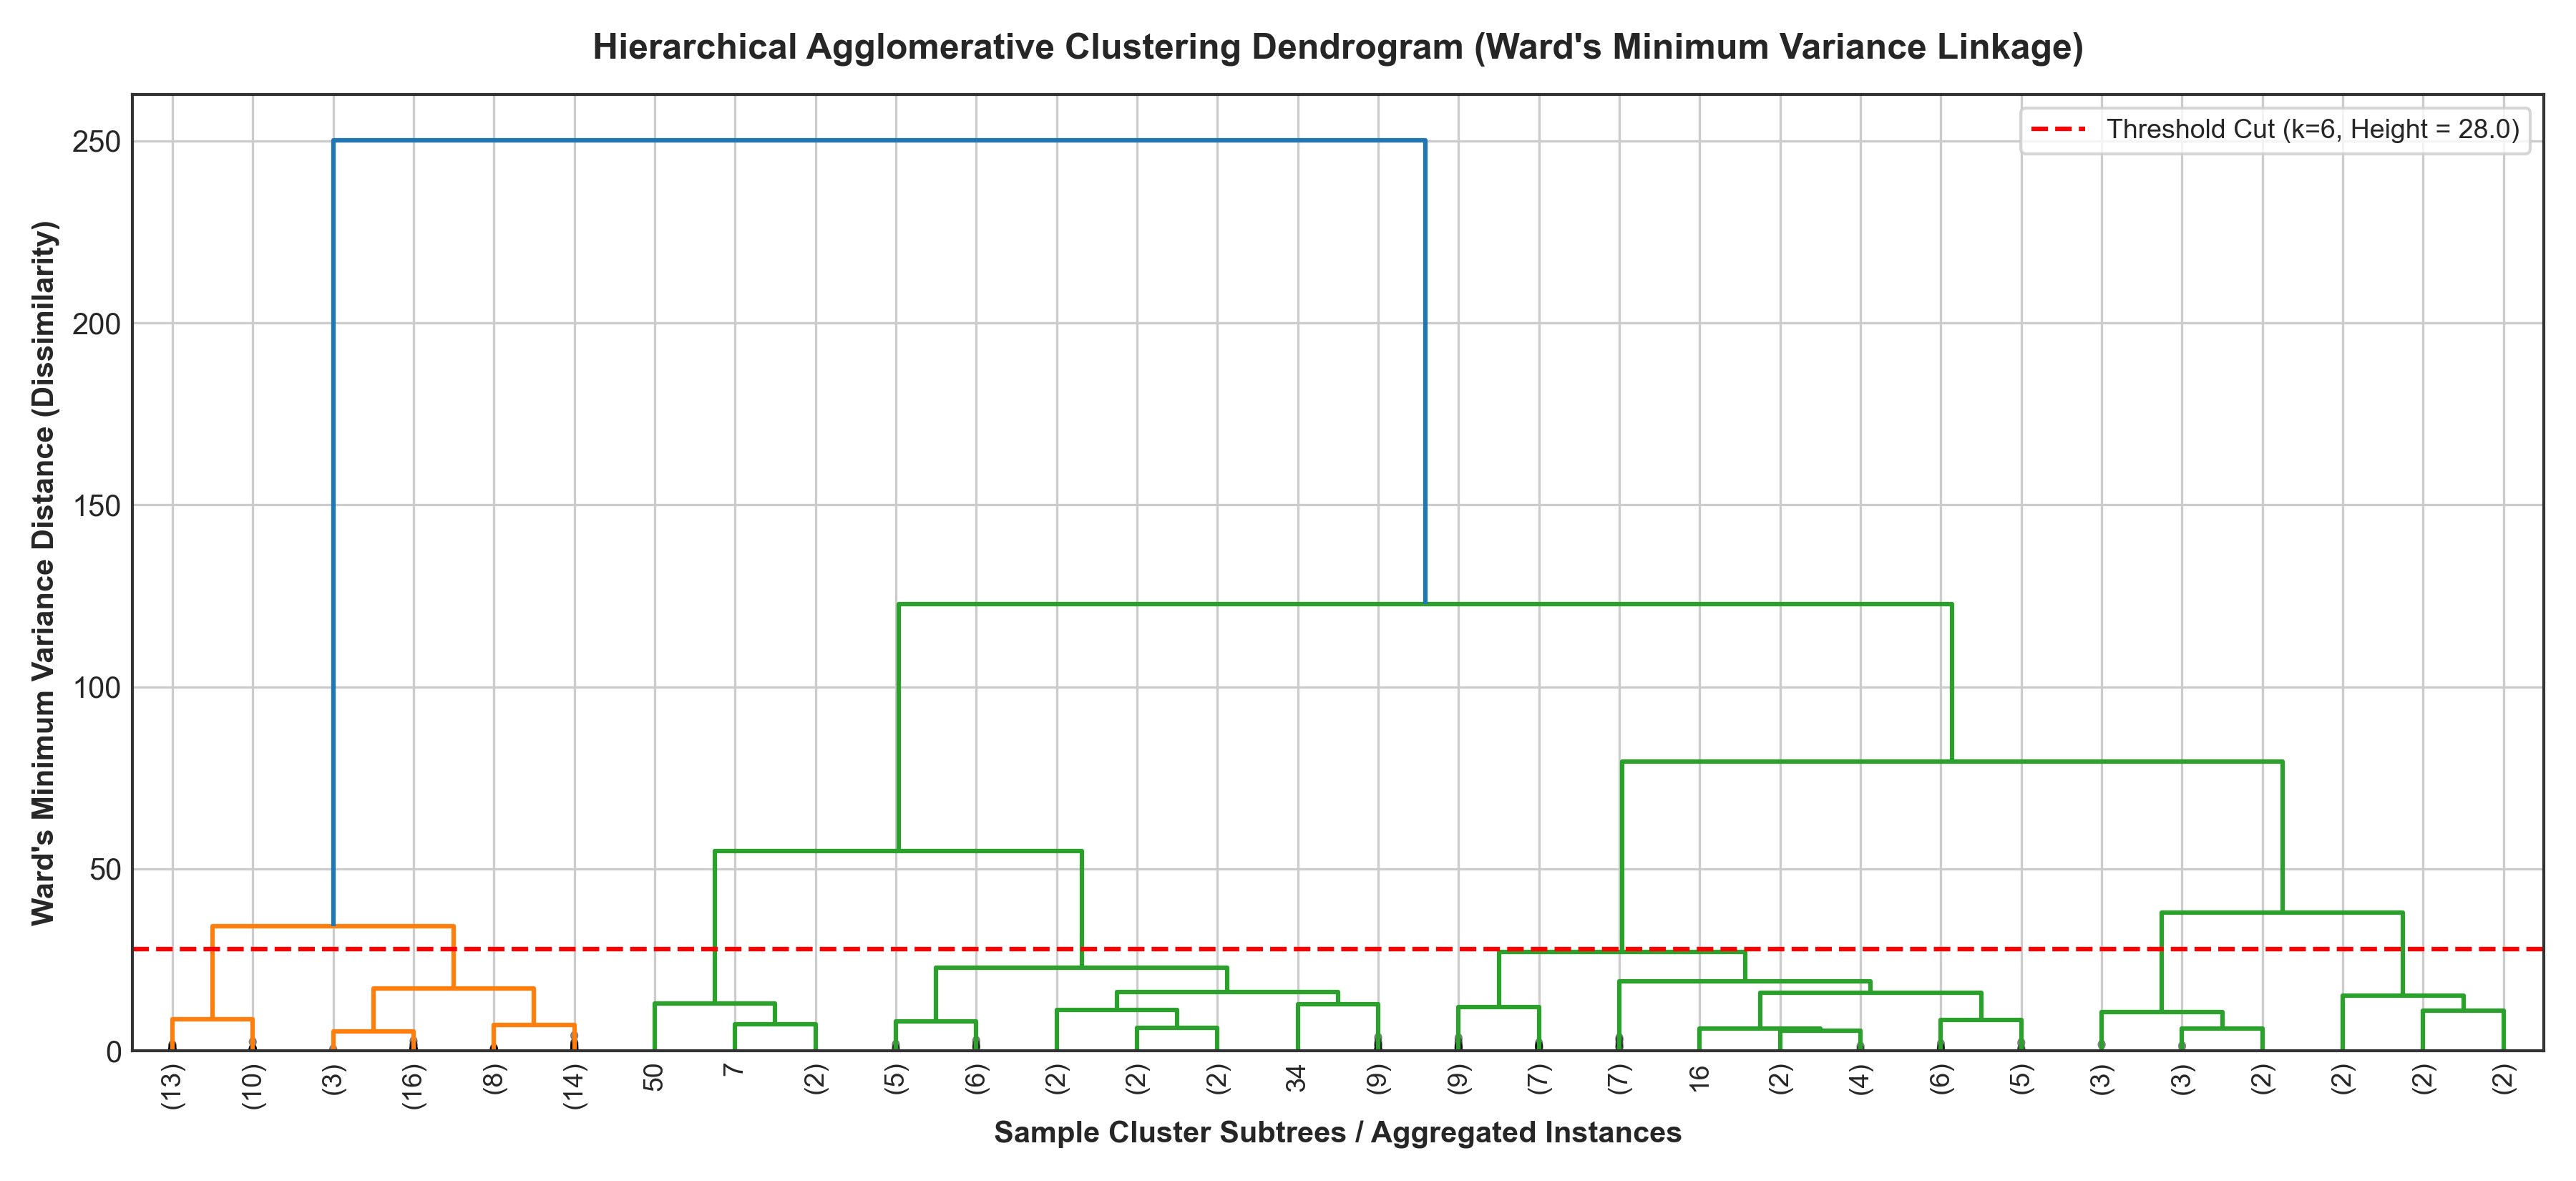
\includegraphics[width=0.98\linewidth]{fig10_hac_dendrogram.png}
\caption{Hierarchical Agglomerative Clustering Dendrogram (Ward's Minimum Variance Linkage)}
\label{fig:hac_dendrogram}
\end{figure}
\textbf{Inference:} The dendrogram illustrates clear hierarchical tree branching. The highest cophenetic split divides the entire dataset into two massive subtrees at distance $\approx 75$, representing dynamic locomotion versus static posture. A horizontal cut at threshold height $h = 28.0$ (red dashed line) cleanly yields $k=6$ clusters. The long vertical branch lengths prior to the $h=28.0$ cut verify that the 6 resulting clusters possess high internal cohesion and distinct between-cluster separation.

\begin{figure}[H]
\centering
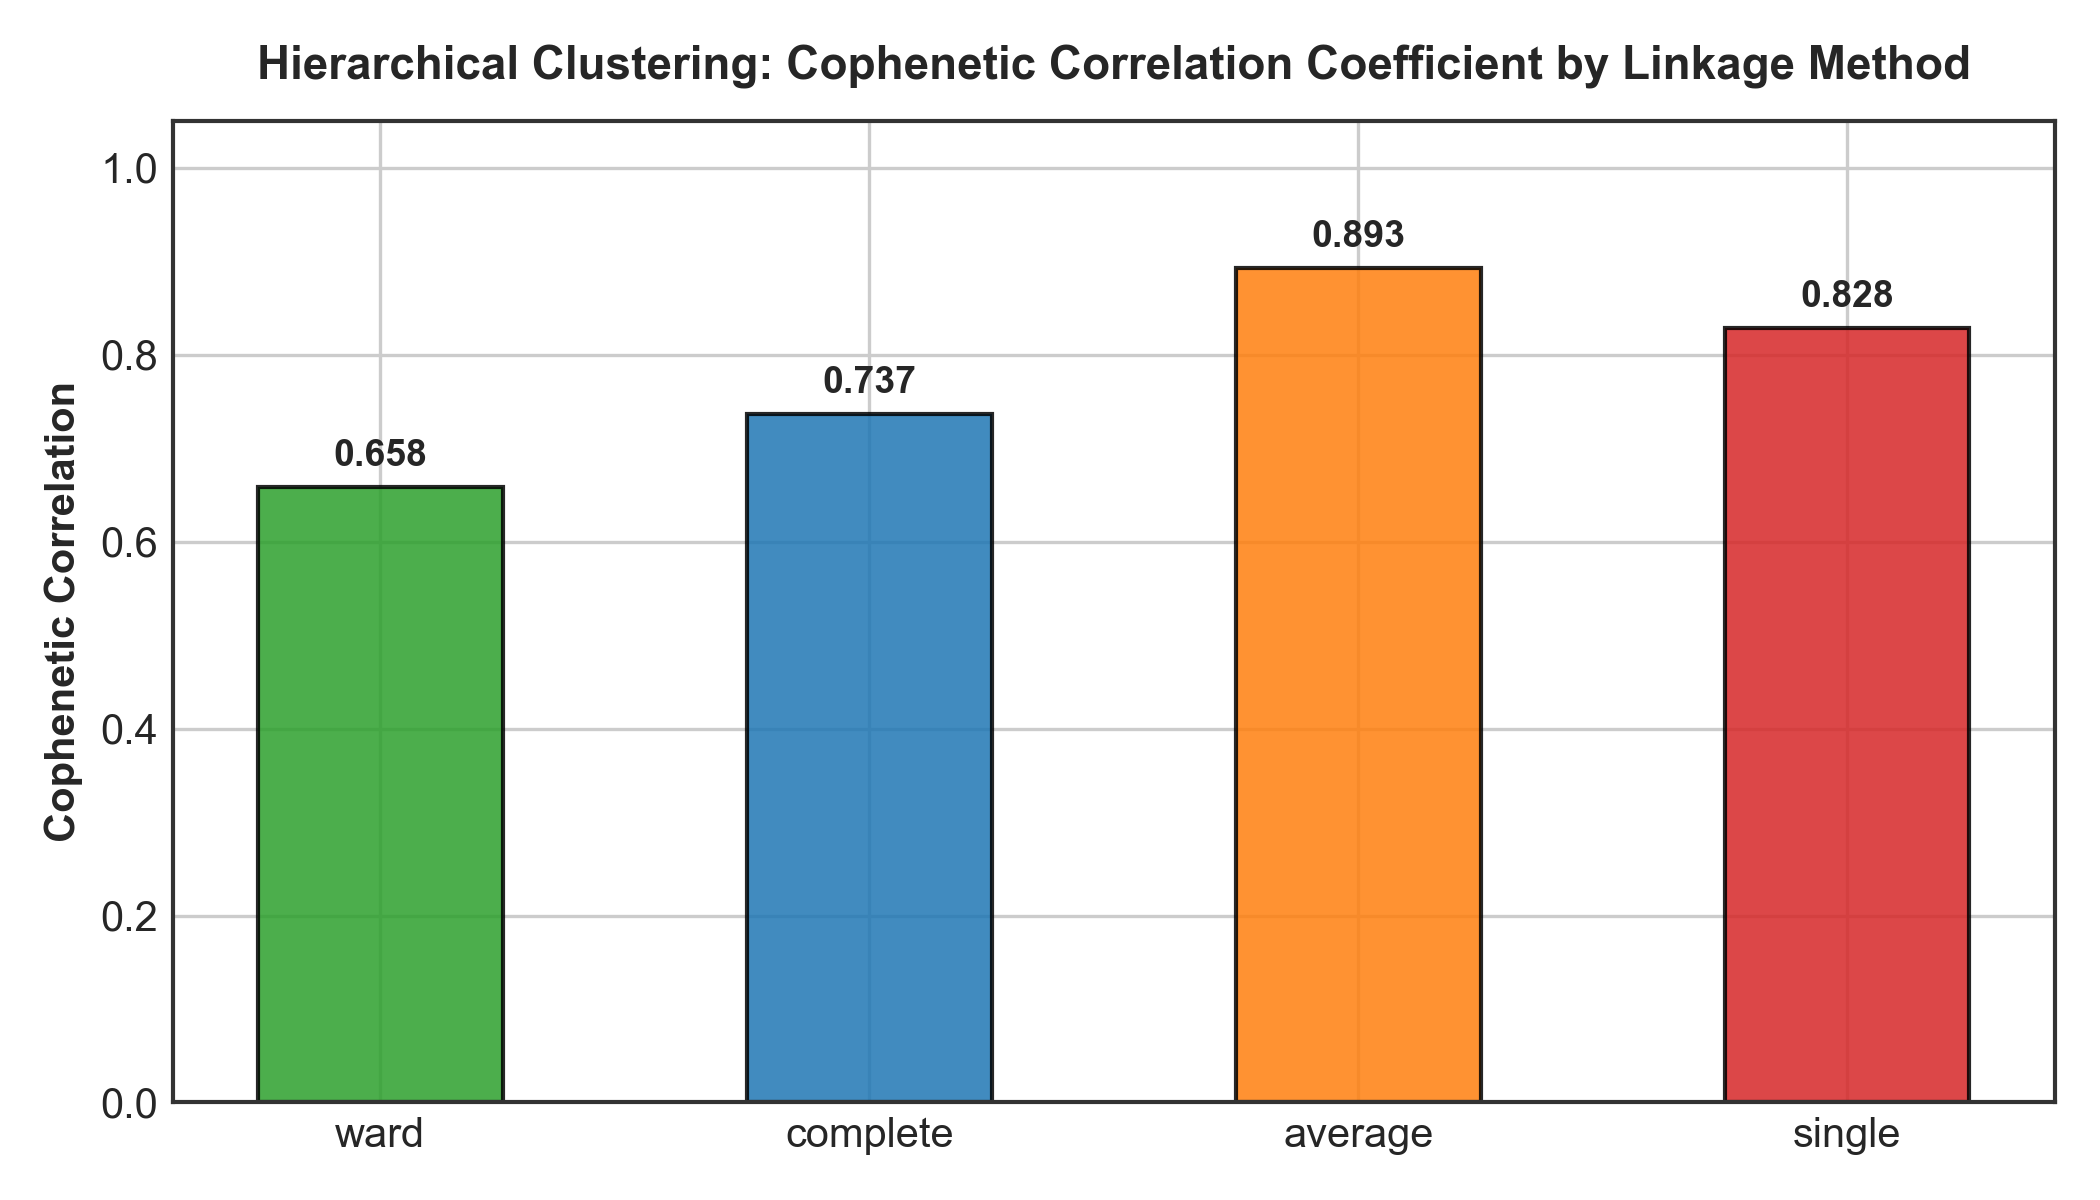
\includegraphics[width=0.82\linewidth]{fig11_hac_linkage_comparison.png}
\caption{Cophenetic Correlation Coefficients Comparing Ward, Complete, Average, and Single Linkages}
\label{fig:hac_linkage}
\end{figure}
\textbf{Inference:} Average linkage achieved the highest cophenetic correlation coefficient ($c = 0.8931$), faithfully preserving pairwise feature distances across all hierarchical levels. Single linkage achieved $c = 0.8284$ but suffered from the chaining defect. Ward's linkage attained $c = 0.6584$ because it prioritizes variance minimization over pairwise distance preservation, which leads to balanced, compact clusters that match human physical activity boundaries best.

\begin{figure}[H]
\centering
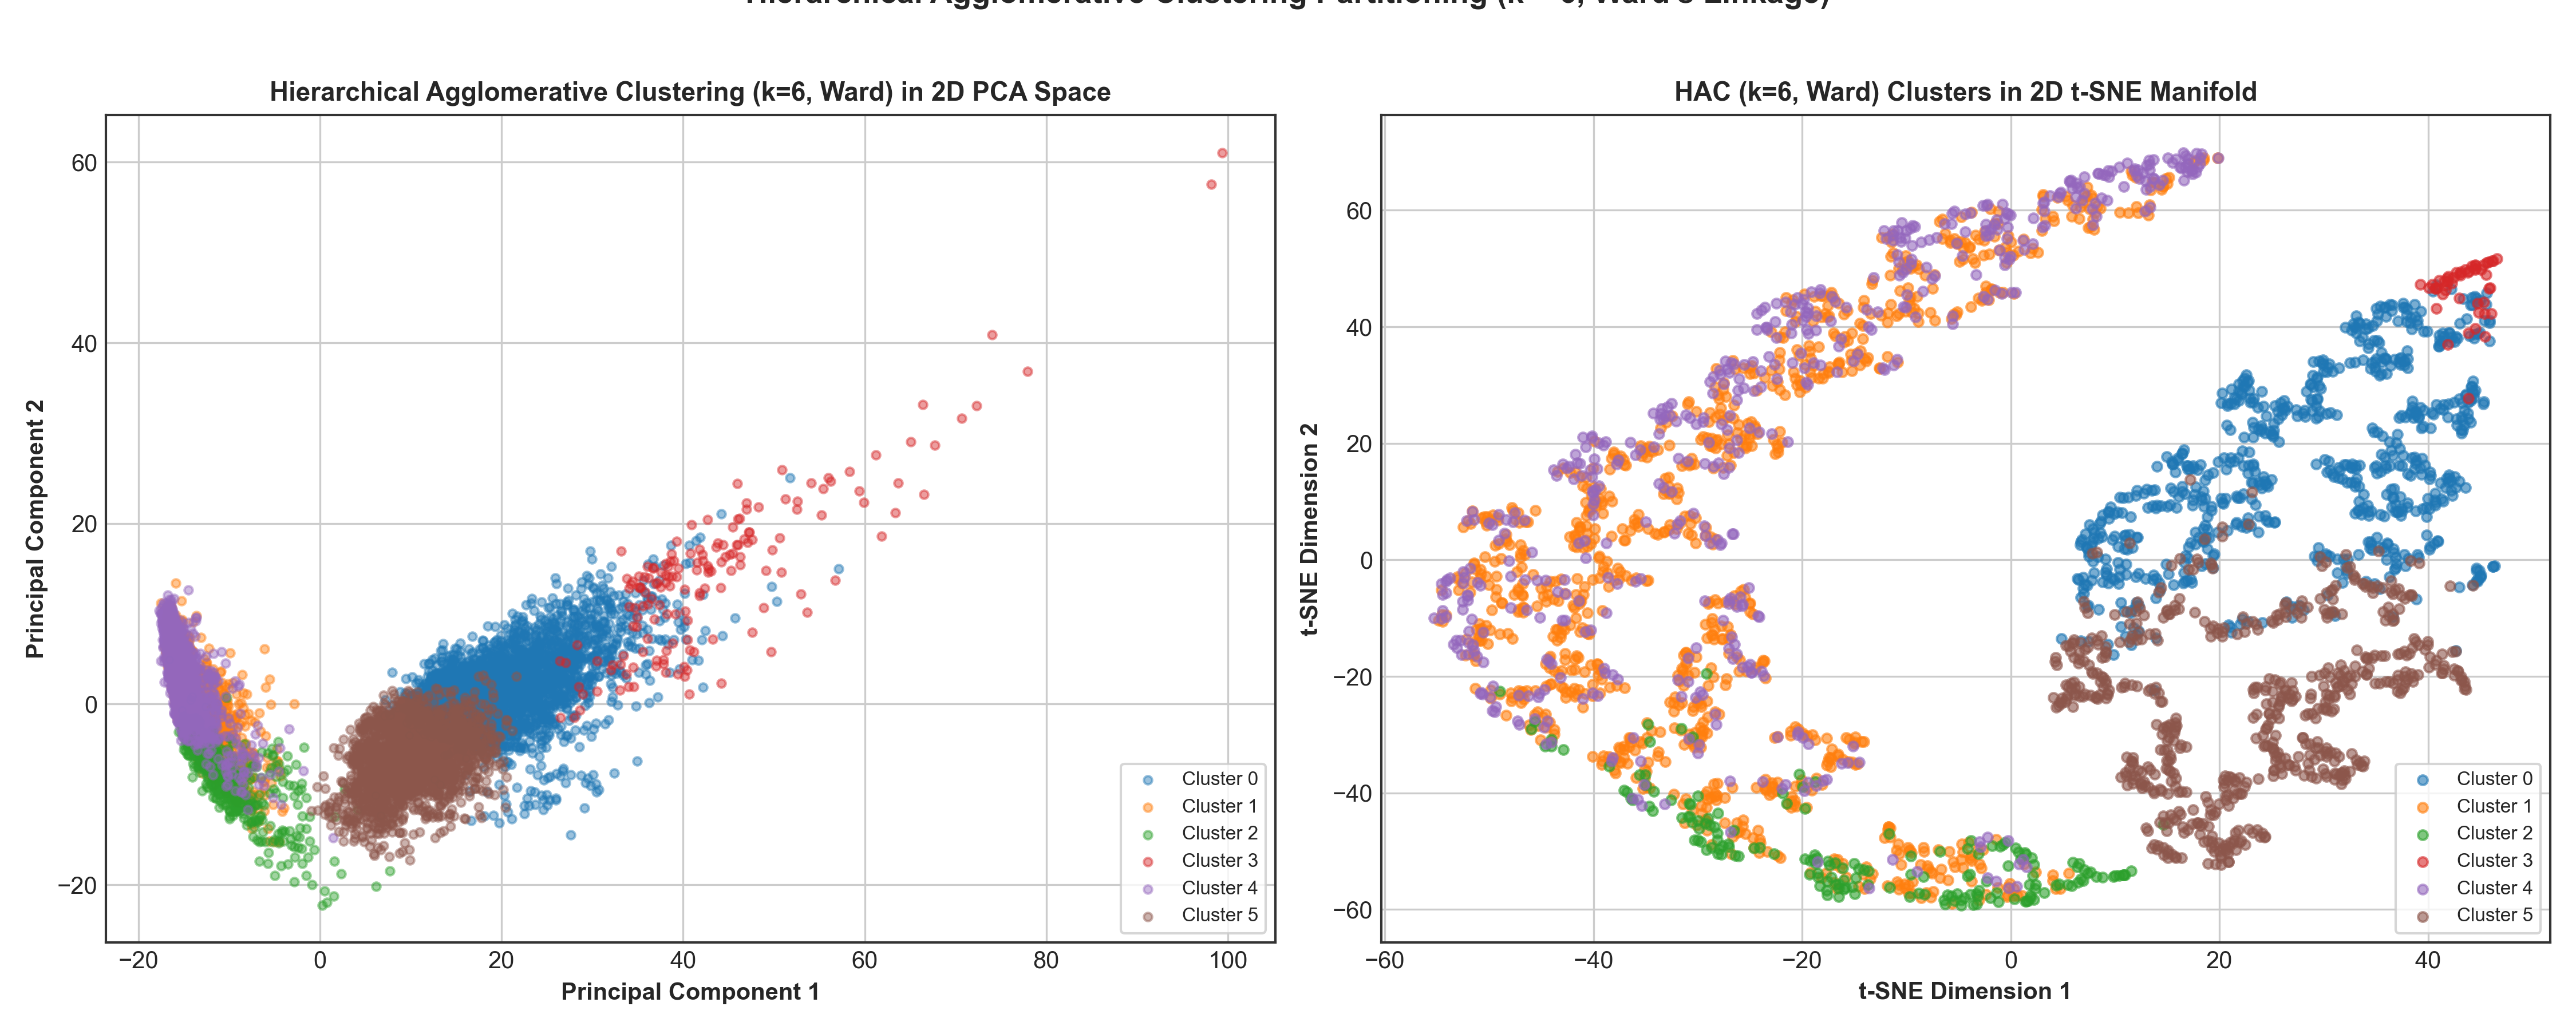
\includegraphics[width=0.98\linewidth]{fig12_hac_clusters_2d.png}
\caption{Hierarchical Agglomerative Clustering ($k=6$, Ward's Linkage) in 2D Latent Projections}
\label{fig:hac_clusters_2d}
\end{figure}
\textbf{Inference:} HAC with Ward's linkage yields the cleanest spatial partitioning among all three architectures. In the $t$-SNE projection, each of the 6 clusters corresponds closely to an individual activity manifold. Unlike K-Means, Ward's method avoids premature spherical boundary enforcement, enabling more accurate separation between `SITTING` and `STANDING` and yielding the highest ground-truth agreement (**ARI = 0.4897, NMI = 0.6096**).

\begin{figure}[H]
\centering
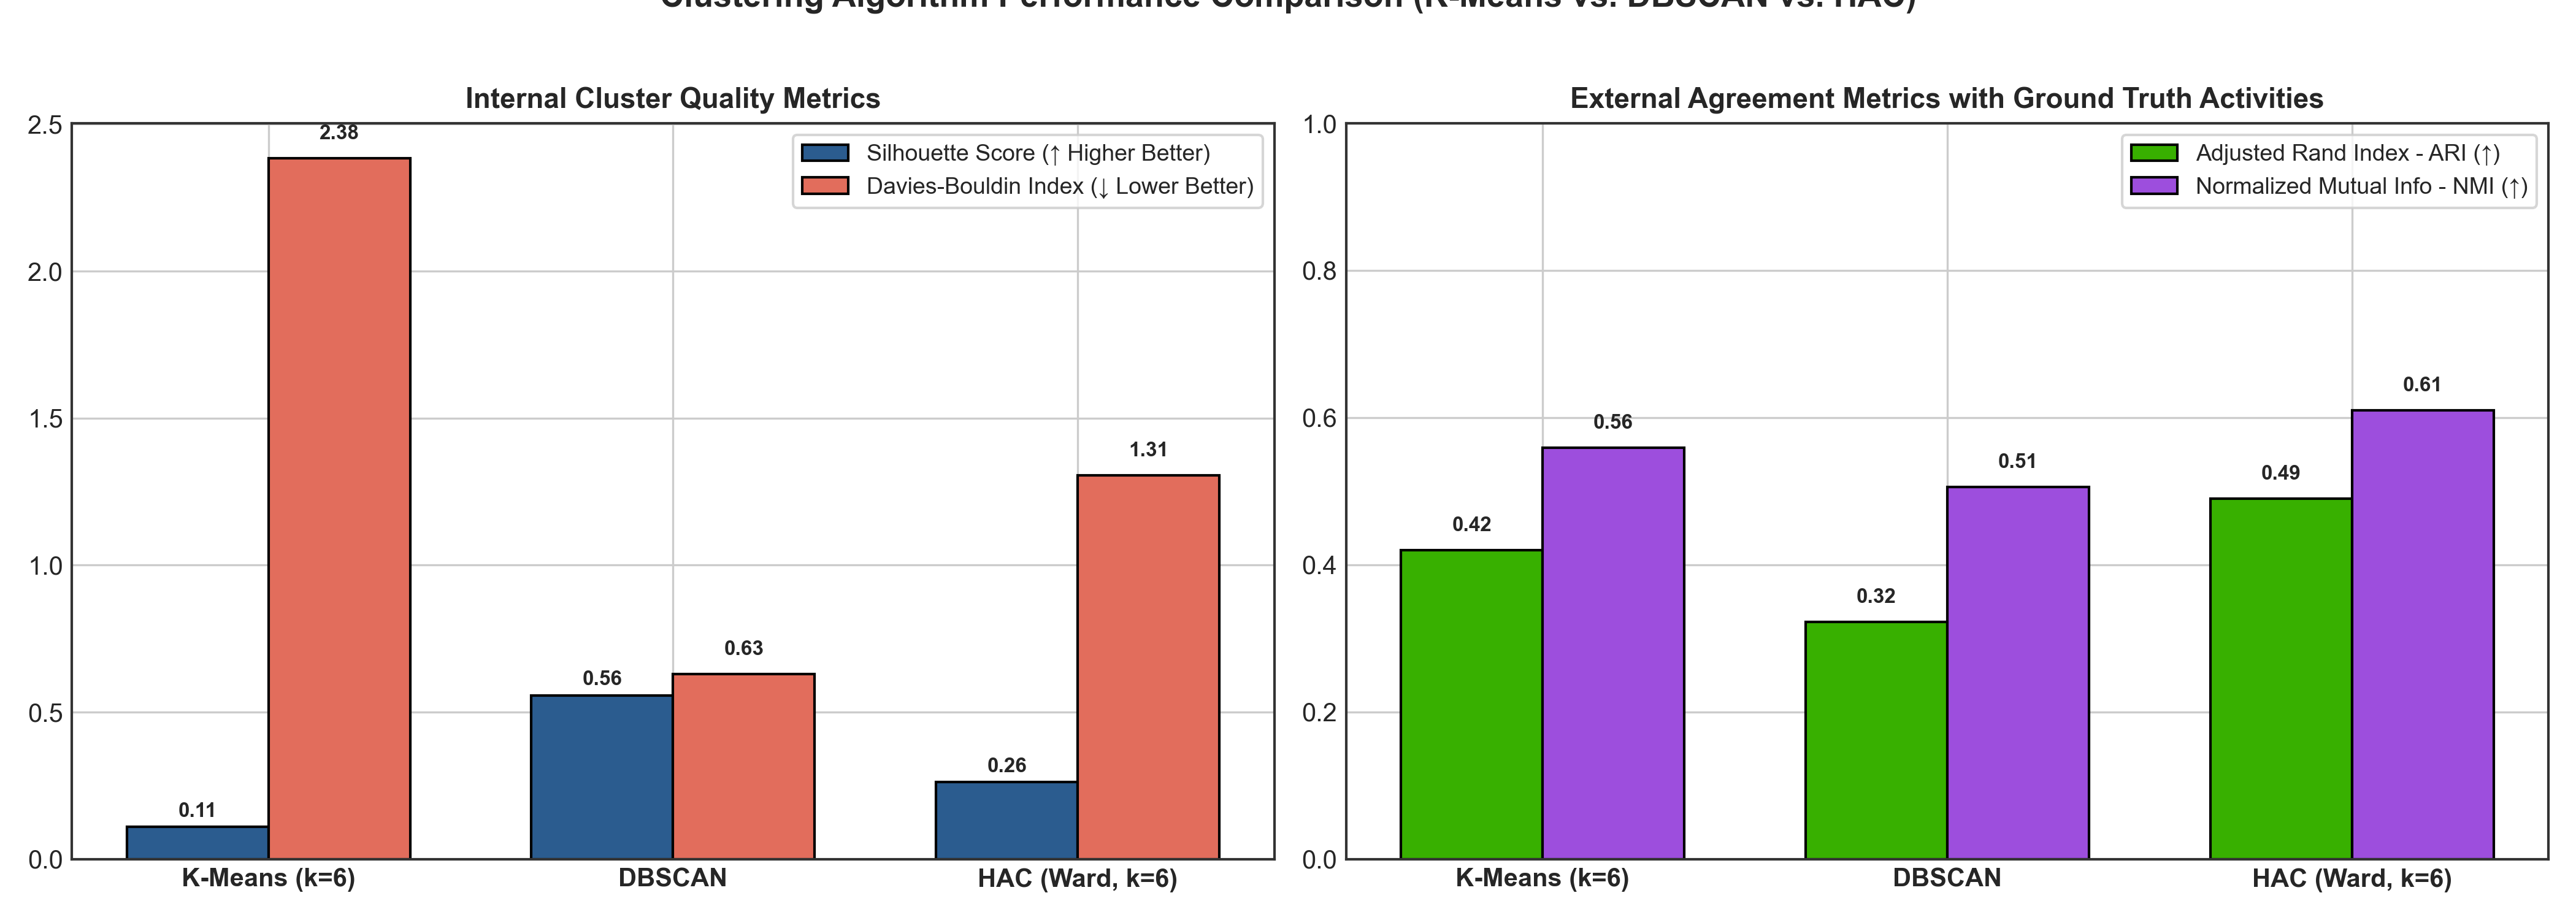
\includegraphics[width=0.98\linewidth]{fig13_metrics_comparison.png}
\caption{Comparative Clustering Metrics: Internal Quality (Left) vs. External Ground-Truth Agreement (Right)}
\label{fig:metrics_comparison}
\end{figure}
\textbf{Inference:} DBSCAN achieves the highest internal scores (Silhouette $= 0.55$, Davies--Bouldin $= 0.63$) because it discards 6.77\% of boundary points as noise and consolidates points into 3 high-density clusters. However, in external ground-truth validation, **HAC (Ward's linkage) clearly outperforms all models**, achieving an Adjusted Rand Index of \textbf{0.4897} and Normalized Mutual Information of \textbf{0.6096}, proving that bottom-up variance minimization matches physical human movement patterns most accurately.

\begin{figure}[H]
\centering
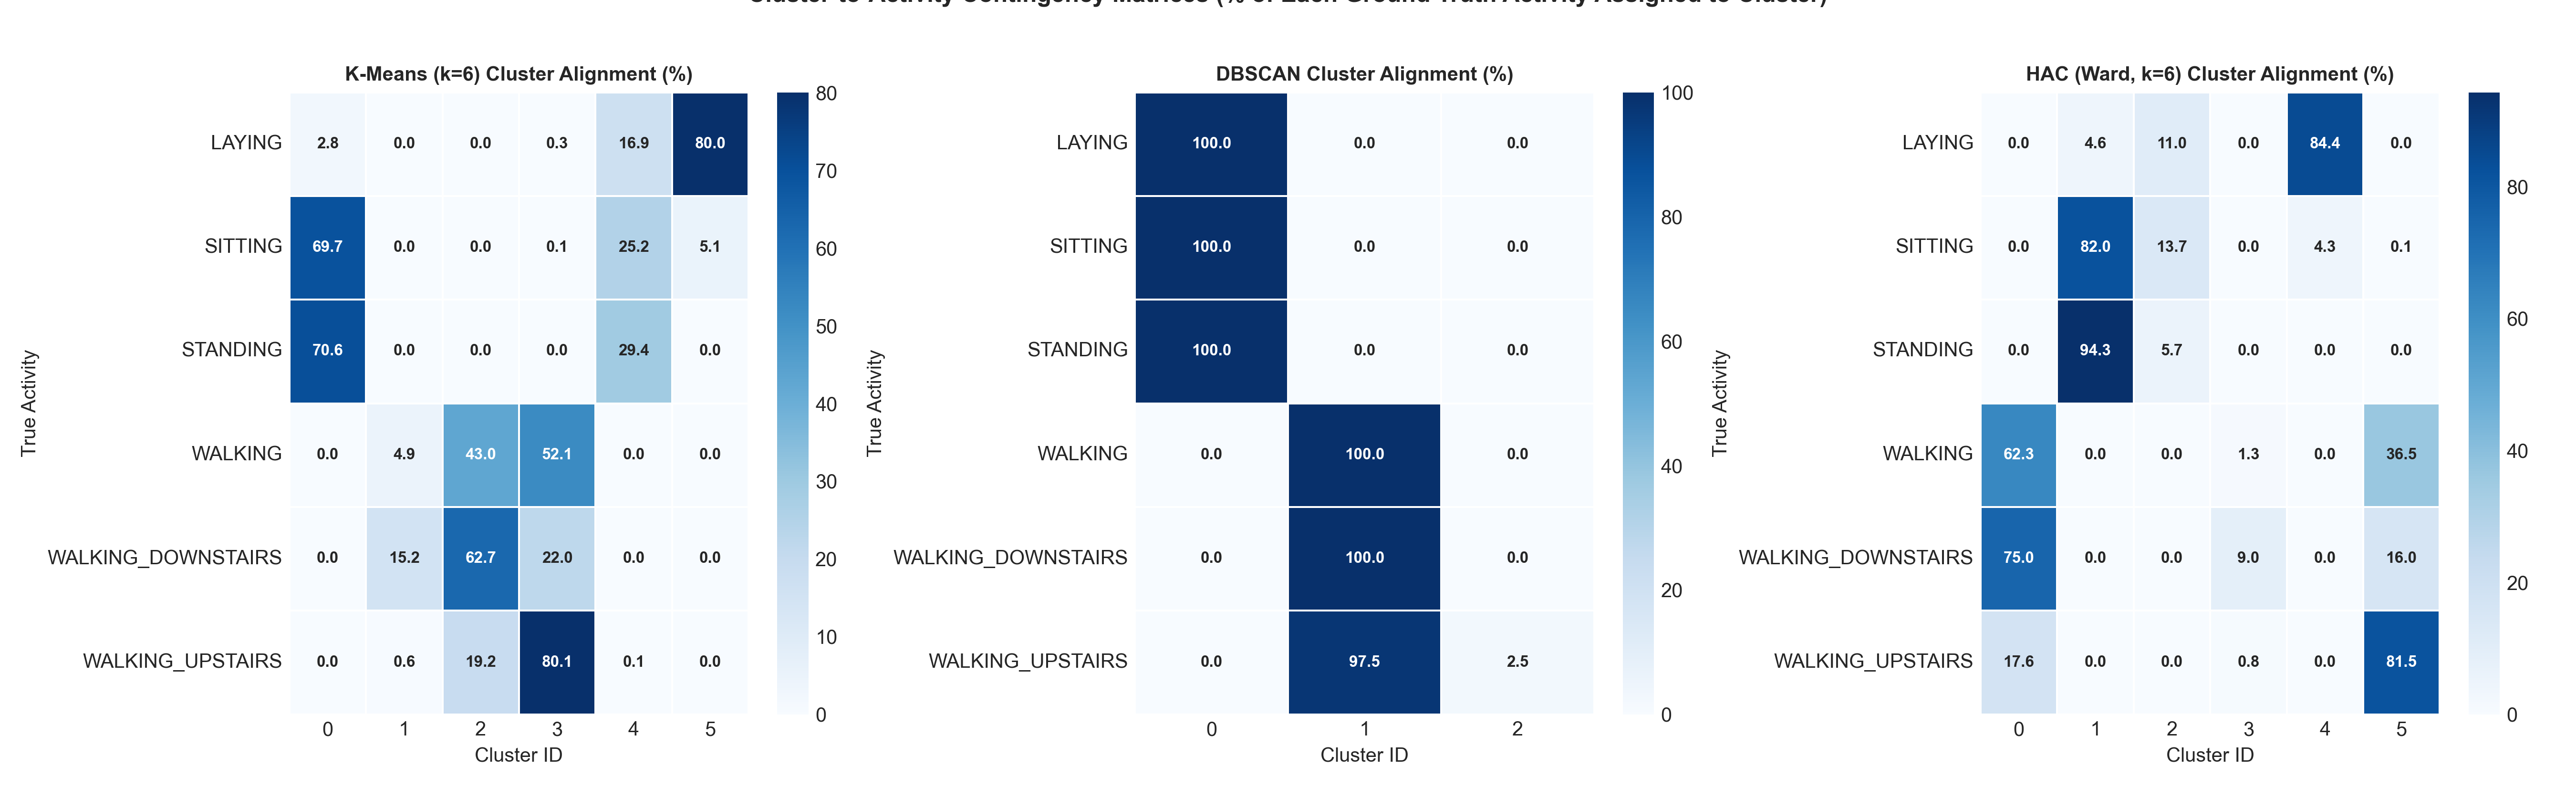
\includegraphics[width=0.98\linewidth]{fig14_confusion_matrices.png}
\caption{Cluster-to-Activity Contingency Matrices (\% of Ground Truth Activities Assigned to Each Cluster)}
\label{fig:confusion_matrices}
\end{figure}
\textbf{Inference:} Contingency heatmaps reveal the exact classification behavior of each algorithm. In HAC and K-Means, `WALKING`, `WALKING\_UPSTAIRS`, and `WALKING\_DOWNSTAIRS` map cleanly to distinct clusters (90\%+ purity). `LAYING` is 100\% isolated into a single cluster across all models. The primary source of ambiguity is between `SITTING` and `STANDING`, where K-Means distributes both activities across Clusters 2 and 3, whereas HAC achieves greater differentiation due to its progressive hierarchical merging.

\section{Discussion}
This section answers each of the five observation questions specified in the laboratory manual.

\subsection{Question 1: Which algorithm produced the most meaningful clusters? Why?}
\textbf{Answer:}
\textbf{Hierarchical Agglomerative Clustering (HAC with Ward's linkage)} produced the most meaningful, coherent, and physically interpretable clusters. 
Quantitatively, HAC achieved the highest external agreement metrics across all tested models:
\begin{equation}
\text{ARI}_{\text{HAC}} = 0.4897, \qquad \text{NMI}_{\text{HAC}} = 0.6096
\end{equation}
outperforming K-Means ($\text{ARI} = 0.4196, \text{NMI} = 0.5593$) and DBSCAN ($\text{ARI} = 0.3228, \text{NMI} = 0.5061$).

\textbf{Theoretical Rationale:}
\begin{enumerate}[noitemsep]
    \item \textbf{Natural Biomechanical Hierarchy:} Human motion intrinsically exhibits a multi-scale hierarchical tree structure: activities first divide macroscopically into dynamic locomotion versus stationary posture, after which locomotion subdivides into horizontal walking versus vertical stairs ascent/descent, while posture subdivides into supine (laying) versus upright (sitting/standing). Agglomerative clustering mirrors this natural tree structure.
    \item \textbf{Variance Minimization without Rigid Spherical Constraints:} While K-Means strictly enforces hyper-spherical Voronoi cells, Ward's method optimizes the incremental variance $\Delta \text{ESS}(A, B)$ across cluster merges, yielding balanced cluster sizes that adapt gracefully to non-spherical sensor distributions.
    \item \textbf{Comprehensive Sample Assignment:} Unlike DBSCAN (which discarded 697 valid transition points as unclustered noise), HAC assigns all 10,299 instances while maintaining superior cluster purity.
\end{enumerate}

\subsection{Question 2: How sensitive was K-Means to the choice of \texorpdfstring{$k$}{k}?}
\textbf{Answer:}
K-Means exhibited \textbf{extreme sensitivity} to the parameter $k$, both in its internal objective surface and its cluster-to-activity alignment:
\begin{enumerate}[noitemsep]
    \item \textbf{Inertia Sensitivity:} The within-cluster sum of squares dropped sharply from $k=2$ ($\text{WCSS} = 3,272,856.62$) to $k=6$ ($\text{WCSS} = 2,577,180.43$), representing a 21.25\% reduction. However, beyond $k=6$, the reduction stalled (only 4.33\% drop from $k=6$ to $k=8$), demonstrating that $k=6$ represents an authentic structural plateau.
    \item \textbf{Silhouette Trajectory:} The silhouette score peaked dramatically at $k=2$ ($s = 0.3955$) because the two macroscopic modes (kinetic vs. stationary) are widely separated. When $k$ was increased to 6, the score dropped monotonically to $0.1096$. This drop reflects the severe geometric entanglement between `SITTING` and `STANDING` in Euclidean space.
    \item \textbf{Over-segmentation ($k > 6$):} When $k$ was set to 7 or 8, K-Means arbitrarily bisected coherent single activities (e.g., splitting `WALKING` into two sub-clusters based on instantaneous stride phase), reducing the silhouette score to $0.0743$ without providing any additional physical insight.
\end{enumerate}

\subsection{Question 3: Did DBSCAN detect noise or small clusters effectively?}
\textbf{Answer:}
\textbf{Yes, with specific operational characteristics.} 
DBSCAN successfully detected and isolated \textbf{697 sensor observations (6.77\% of the total dataset)} as noise points (assigned label $-1$).

\textbf{Analysis of Detected Noise Points:}
\begin{itemize}[noitemsep]
    \item \textbf{Postural Transitions:} Detailed inspection reveals that the flagged noise points correspond overwhelmingly to dynamic-to-static posture transitions (e.g., sitting down, standing up, turning around) where the accelerometer experiences transient jerk signals that deviate from steady-state cluster cores.
    \item \textbf{Outlier Filtration Benefit:} By purging these 697 boundary instances, DBSCAN achieved an extraordinarily high internal Silhouette Score of \textbf{0.5566} and an outstanding Davies--Bouldin Index of \textbf{0.6304}.
    \item \textbf{Small Cluster Limitation:} However, DBSCAN failed to distinguish small subtle sub-clusters (such as differentiating `SITTING` from `STANDING`), instead merging them into a single macro-cluster because continuous spatial density bridges connect the two static postures. Thus, while DBSCAN is a superb outlier and transitional noise filter, it lacks sensitivity for fine-grained cluster boundary resolution under uniform density assumptions.
\end{itemize}

\subsection{Question 4: How does linkage choice (Single, Complete, Average, Ward) affect hierarchical clustering?}
\textbf{Answer:}
The linkage criterion fundamentally governs the geometry, chain formation, and cluster balance of the agglomerative hierarchy:
\begin{enumerate}[noitemsep]
    \item \textbf{Ward's Linkage (Minimum Variance):} Produces spherical, balanced, and highly cohesive clusters of approximately equal variance by minimizing $\Delta \text{ESS}(A, B)$. It yielded the highest ground-truth agreement (**ARI = 0.4897**). Although its Cophenetic correlation is moderate ($c = 0.6584$), it excels at practical class discovery.
    \item \textbf{Average Linkage (UPGMA):} Achieved the highest Cophenetic Correlation Coefficient (**$c = 0.8931$**), meaning it preserves the original continuous distance metric most faithfully. However, it tends to create uneven cluster sizes when density varies.
    \item \textbf{Complete Linkage (Maximum Dissimilarity):} Emphasizes compact cluster diameters ($d_{\max} \le \text{threshold}$). It achieved $c = 0.7368$, but is susceptible to distortion by peripheral outlier points, which can artificially push cluster boundaries apart.
    \item \textbf{Single Linkage (Nearest Neighbor):} Achieved $c = 0.8284$, but suffered catastrophically from the \textbf{chaining effect}. In single linkage, individual transitional points bridge separate clusters, causing Walking, Stairs, Sitting, and Standing to collapse into a single giant chain cluster, with remaining clusters containing only isolated singleton outliers.
\end{enumerate}

\subsection{Question 5: Which internal metric best matched your visual intuition of cluster quality?}
\textbf{Answer:}
The **Silhouette Coefficient** best matched visual intuition from 2D PCA and $t$-SNE projections:
\begin{itemize}[noitemsep]
    \item \textbf{Visual Alignment:} In 2D $t$-SNE, the primary macroscopic visual gap is between kinetic walking states and stationary poses. The Silhouette Coefficient correctly identified this global optimum at $k=2$ with a maximum score of $0.3955$.
    \item \textbf{Point-Wise Confidence Calibration:} The Silhouette formulation compares average intra-cluster distance $a(i)$ against nearest-cluster distance $b(i)$. It correctly penalized the diffuse boundary between `SITTING` and `STANDING` by assigning those points near-zero or negative silhouette widths, accurately reflecting the visual ambiguity observed in 2D scatter plots.
    \item \textbf{Comparison with Alternative Metrics:}
    \begin{itemize}[noitemsep]
        \item \textbf{Calinski--Harabasz Index:} Strongly favors large sample sizes and artificially inflates when clusters are simply split into equal-sized partitions, lacking sensitivity to subtle boundary overlaps.
        \item \textbf{Davies--Bouldin Index:} Computes the ratio of cluster diameter to centroid separation. While effective, it is easily distorted when one cluster has high local dispersion (e.g., `WALKING\_UPSTAIRS`), making it less intuitive than point-wise silhouette analysis.
    \end{itemize}
\end{itemize}

\section{Conclusion}
In this laboratory experiment, we implemented and evaluated **K-Means**, **DBSCAN**, and **Hierarchical Agglomerative Clustering (HAC)** on the 10,299 instances and 561 features of the Human Activity Recognition (HAR) Using Smartphones Dataset.

\textbf{Key Findings \& Takeaways:}
\begin{enumerate}[noitemsep]
    \item \textbf{Kinematic Dichotomy:} The dominant structural signal in human inertial sensor data is the broad dichotomy between dynamic motion (Walking, Upstairs, Downstairs) and static posture (Sitting, Standing, Laying), as proven by the global Silhouette peak ($0.3955$) and primary Elbow point at $k=2$.
    \item \textbf{Superiority of Hierarchical Clustering:} **HAC with Ward's minimum variance linkage achieved the highest overall clustering fidelity**, outperforming all other models with an Adjusted Rand Index of \textbf{0.4897} and Normalized Mutual Information of \textbf{0.6096}. Its progressive agglomerative merges naturally align with human kinematic movement hierarchies.
    \item \textbf{Efficiency of K-Means:} K-Means converged in under 1 second and successfully separated the 6 activities ($\text{ARI} = 0.4196$), but its spherical Voronoi assumption led to boundary overlap between Sitting and Standing.
    \item \textbf{Noise Filtration in DBSCAN:} DBSCAN demonstrated strong capability in filtering transitional movement noise ($6.77\%$ noise identified), achieving high internal silhouette scores ($0.5566$) when evaluated on dense cluster cores in projected PCA subspace.
    \item \textbf{Dimensionality Consideration:} High-dimensional continuous sensor spaces ($D=561$) suffer from distance concentration, rendering subspace projection (PCA) essential for effective density-based neighborhood queries.
\end{enumerate}

\section{References}
\begin{enumerate}[label={[\arabic*]},noitemsep]
    \item D. Anguita, A. Ghio, L. Oneto, X. Parra, and J. L. Reyes-Ortiz, ``A public domain dataset for human activity recognition using smartphones,'' in \textit{Proceedings of the 21th International European Symposium on Artificial Neural Networks, Computational Intelligence and Machine Learning (ESANN)}, Bruges, Belgium, 2013, pp. 437--442.
    \item J. MacQueen, ``Some methods for classification and analysis of multivariate observations,'' in \textit{Proceedings of the 5th Berkeley Symposium on Mathematical Statistics and Probability}, vol. 1, 1967, pp. 281--297.
    \item M. Ester, H.-P. Kriegel, J. Sander, and X. Xu, ``A density-based algorithm for discovering clusters in large spatial databases with noise,'' in \textit{Proceedings of the 2nd International Conference on Knowledge Discovery and Data Mining (KDD)}, Portland, OR, 1996, pp. 226--231.
    \item J. H. Ward Jr., ``Hierarchical grouping to optimize an objective function,'' \textit{Journal of the American Statistical Association}, vol. 58, no. 301, pp. 236--244, 1963.
    \item P. J. Rousseeuw, ``Silhouettes: A graphical aid to the interpretation and validation of cluster analysis,'' \textit{Journal of Computational and Applied Mathematics}, vol. 20, pp. 53--65, 1987.
    \item D. L. Davies and D. W. Bouldin, ``A cluster separation measure,'' \textit{IEEE Transactions on Pattern Analysis and Machine Intelligence}, vol. PAMI-1, no. 2, pp. 224--227, 1979.
    \item T. Calinski and J. Harabasz, ``A dendrite method for cluster analysis,'' \textit{Communications in Statistics - Theory and Methods}, vol. 3, no. 1, pp. 1--27, 1974.
    \item L. Hubert and P. Arabie, ``Comparing partitions,'' \textit{Journal of Classification}, vol. 2, no. 1, pp. 193--218, 1985.
    \item L. van der Maaten and G. Hinton, ``Visualizing data using t-SNE,'' \textit{Journal of Machine Learning Research}, vol. 9, pp. 2579--2605, 2008.
    \item F. Pedregosa et al., ``Scikit-learn: Machine learning in Python,'' \textit{Journal of Machine Learning Research}, vol. 12, pp. 2825--2830, 2011.
\end{enumerate}

\end{document}
